\documentclass [12pt,fleqn]{article}

\usepackage{color}
\usepackage{amssymb}
\usepackage[font={small,it}]{caption}
\usepackage{bm}
\usepackage{draftwatermark}
\usepackage{epsf,graphicx}
\usepackage{psfrag}
\usepackage{textcomp}
\usepackage{float}
\usepackage{amsmath}
\usepackage{siunitx}
\usepackage[mathscr]{euscript}
\usepackage{color}
\usepackage{verbatim}
\usepackage{authblk}
\usepackage{lineno}

\usepackage{lineno}
\linenumbers

\SetWatermarkText{Draft}
\SetWatermarkScale{5}

\usepackage[a4paper,bindingoffset=0.2in,%
            left=1in,right=1in,top=1in,bottom=1in,%
            footskip=.25in]{geometry}

%\usepackage{setspace}
%\doublespacing
%\usepackage[cal=mathpi,
%calscaled=.94,
%bb=ams,
%frak=mma,
%frakscaled=.97,
%scr=rsfs]{mathalfa}

\makeatletter
\g@addto@macro\@floatboxreset\centering
\makeatother
            

%\topmargin     -0.60in  % (adjusted for printer bias) 
%\headheight      .00in  % (no headers) 
%\headsep         .50in  % (top margin + headers + skip) 
\textheight     9.50in  % (instructions: 9 1/8'' min, 9 7/16'' max) 
%\textwidth      7.00in  % 2*3.33 + .33 = 6.99 
%\oddsidemargin  0.3125in  % (subtracted 1inch bias) 
%\evensidemargin 0.3125in  
\parindent .0in 
\parskip 10pt 

\newcommand*{\matminus}{%
  \leavevmode
  \hphantom{0}%
  \llap{%
    \settowidth{\dimen0 }{$0$}%
    \resizebox{1.1\dimen0 }{\height}{$-$}%
  }%
}

\renewcommand*{\thefootnote}{\fnsymbol{footnote}}
\newcommand{\angstrom}{\textup{\AA}}


\font \bigtenrm=cmmi10 scaled\magstep2 
\def \be {\begin{equation}} 
\def \ee {\end{equation}} 
\def \beq {\begin{eqnarray}} 
\def \eeq {\end{eqnarray}} 

\title{Wide-angle correlated X-ray scattering from nanoparticles is consistent with an atomic twinning model}
%\title{Wide-angle correlated X-ray scattering from gold nanoparticles demonstrated precise agreement with an atomic twinning model}

\author{Derek Mendez}
\author[1]{Herschel Watkins}
\author[1]{Shenglan Qiao}
\author[1]{Kevin S. Raines}
\author[2]{ Thomas J. Lane}
\author[1]{Gundolf Schenk}
\author[4]{Kensuke Tono}
\author[4]{Yasumasa Joti}
\author[3]{Makina Yabashi}
\author[2]{Daniel Ratner}
\author[1,2]{Sebastian Doniach}

\affil [1]{Stanford University Department of Applied Physics, Stanford, CA 94305}
\affil [2]{SLAC National Accelerator Laboratory, Menlo Park, CA 94025}
\affil [3]{RIKEN SPring-8 Center, Kouto 1-1-1, Sayo, Hyogo 679-5148, Japan}
\affil [4]{Japan Synchrotron Radiation Research Institute (JASRI), Kouto 1-1-1, Sayo, Hyogo 679-5198, Japan}

\renewcommand\Authands{ and }

\begin{document}
\maketitle
\delimitershortfall=-1pt

\begin{center}
\section*{Abstract}
\end{center}
We report on measurements of angular intensity correlations from gold nanoparticle scattering at the Spring-8 Angstrom Compact Free Electron Laser facility (SACLA). Each wide-angle snapshot captured X-ray scattering from nearly ten thousand gold nanoparticles suspended freely in random orientations. By averaging photon intensity correlations over tens of thousands of snapshots, we observe correlated X-ray scattering (CXS). We separate the measured photon intensities into two groups and find that the resulting CXS signals indicate two populations of nanoparticle domains present in our sample: small, twinned domains (SD) and large, non-twinned domains (LD). Comparing the measured CXS signal of the SDs to that of atomic models and analytical predictions, we resolve a detailed twinning structure. Conversely, the LDs do not show significant indications of twinning. With this result, we demonstrate that CXS analysis can resolve atomic-level information from a three-dimensional, nanoscopic system, even in the presence of significant systematic noise.

\section{Introduction}
Correlated X-ray scattering (CXS), also referred to as fluctuation X-ray scattering, is an emerging field which involves recording many snapshot exposures of an ensemble of randomly oriented mono-dispersed molecules or particles and employing photon intensity correlation analysis to recover the average internal structure of the objects in the random ensemble \cite{kam1977determination}. CXS has potential to reveal the structural properties of proteins and other soft matter without the use of crystallization \cite{saldin2010beyond, saldin2009structure, saldin2010structure, pande2014deducing, schenk2015potential}. 

An obvious precursor to the study of soft matter CXS is that of nanomaterials, in particular those composed of heavy atoms such as gold or silver due to their large atomic scattering cross sections. Experimental work testing CXS has been published on iron-oxide nanorice samples \cite{liu2013three} and lithographically generated dumbbells \cite{chen2012structure}. These experiments used relatively low-angle scattering data, with one or few exposed objects per snapshot. Here we present results of measurements  of three-dimensional suspensions of gold nanoparticles (NPs) measured at wide scattering angles.

NP suspensions are used in chemical catalysis, and their chemical properties are directly related to  the overall shape and atomic structure of the NPs themselves \cite{yacaman1981effect, narayanan2005catalysis, narayanan2004shape}. As such, there is a need for structural characterization methods. Past work describing the thermodynamics and kinetics of NP growth and formation \cite{ino1969stability, marks1983modified, howie1984elastic, marks1984surface, ringe2013kinetic} has revealed that smaller NPs tend to form complicated twinning structures, e.g. decahedral and icosahedral twins \cite{heinemann1979structure, yacaman1979structure, langille2012stepwise, yang1979crystallography, yang1979crystallography2, dai2002shapes}. Previously, twinning has been observed using electron microscopy and tomography \cite{marks1981high, yacaman1992electron, chen2013three}, where one images single NP projections. On the other hand, conventional powder X-ray diffraction measurements, used widely in industry to characterize ensembles of NPs, are isotropic averages and cannot show signs of twinning. In what follows, we will show how CXS distinguishes  twinned from non-twinned NP domains within a sample of gold NPs.

\begin{figure}[H]
\begin{center}
\includegraphics[keepaspectratio]{./Fig1Mar16_lowres.png}
\end{center}
\caption{Cartoon images of the experimental setup and geometry. \emph{(a)} X-ray pulses (orange) exposing a solution of gold nanoparticles. Shown in bright green is the $\{111\}$ Bragg ring. Also shown are two positions along the Bragg ring, $\phi_1$ and $\phi_2$, separated by an angle $\Delta=\pi$. Artwork courtesy of Gregory M. Stewart (SLAC). \emph{(b)} Elastic scattering geometry corresponding to the case when $\Delta = \pi$. Note that $\psi_{\max} < \pi$ at wide angles.}
\label{fig:setup}
\end{figure}

\begin{figure}[H]
\begin{center}
\includegraphics[keepaspectratio]{./Fig2Mar16_lowres.png}
\end{center}
\caption{CXS of the $\{111\}$ Bragg ring simulated for a single- and multi-domain NP. \emph{(a)} The simulated CXS for a non-twinned cuboctahedron gold NP atomic model (Supplementary Section \ref{supp:sim}) . Note that for singe domain gold particles, one would only expect CXS signal at $\cos \psi  = \pm 1/3$, corresponding to the $\{111\}$ interplanar angles of an FCC crystal. We observe this CXS signal from the large, non-twinned domains (LDs).  \emph{(b)} The simulated CXS for a nearest-neighbor-tetrahedron (NNT, outlined in dashed blue). Multi-twinned particles, such as the decahedron shown here are composed of several NNT units. The angular gap in the decahedron results because the tetrahedra are each close packed FCC domains \cite{yang1979crystallography}. The twinning gives rise to additional CXS peaks. We observe this signal from the small, twinned NP domains (SDs) sub-population of our sample.}
\label{fig:contrast}
\end{figure}

\section{Background}
CXS has been extensively explored as a tool to investigate two-dimensional systems \cite{kurta2013xray, schroer2014characteristics, lehmkuhler2014detecting, kurta2012xray, pedrini2013two, saldin2011new}, however in three-dimensional systems, the structural information encoded in the data becomes more difficult to extract using  CXS techniques \cite{elser2011strategies}. If one or few three-dimensional objects are exposed during each snapshot, then one can use symmetry arguments to recover structural information content \cite{kam1980reconstruction, poon2015use, chen2012structure, liu2013three, starodub2012single, saldin2011reconstructing}. When the number of exposed three-dimensional objects increases, one can use the correlated intensities to infer local structural characteristics \cite{wochner2009x, altarelli2010x, kurta2013cross, malmerberg2015operational}, resolve structural changes \cite{pande2015simulations}, and potentially refine atomic models in an iterative procedure \cite{liu2012computation}. In this paper we report on CXS as a tool to investigate a three-dimensional ensemble of gold NPs, where each snapshot is from samples composed of many NPs.

An object in solution exposed to sufficient X-ray flux can scatter photons into at least two directions, $\bm q_1$ and $\bm q_2$. While the orientation of this object can be random, the angle defined by $\bm q_1$ and $\bm q_2$ 

\be \label{cpsi}
\cos \psi = (\bm q_1 \cdot \bm q_2)/(q_1 \, q_2 )
\ee

is not; it is determined by the object's internal atomic structure. A crystalline NP scatters photons into discrete  Bragg vector directions $\bm q_{hkl}$. We define a detector whose pixels correspond to a set of Bragg vectors $\{\bm q\}$. Let $\bm \omega$ be a triple of Euler angles defining an NP orientation relative to some axis (e.g. that of an X-ray beam). An NP at orientation $\omega$ can scatter photons into the detector provided

\be \label{condition}
\bm R_\omega \cdot \bm q_{hkl} \in \{\bm q\}
\ee

where $\bm R_\omega$ is an operator which rotates the NP from some pre-defined arbitrary orientation into $\omega$. We assume a small fraction of NPs in solution are oriented such that condition (\ref{condition}) is met for two Bragg vectors, $\bm q_{hkl}$ and $\bm q_{h'k'l'}$. When one NP is oriented as such, and if it scatters photons into both $\bm q_{hkl}$ and $\bm q_{h'k'l'}$, then these photons are said to be correlated. This double Bragg scattering produces angular intensity correlations between pairs of Bragg vectors in $\{\bm q\}$ whose angular separation $\psi$ is defined by

\be \label{hklcorr}
\cos \psi_{hkl,h'k'l'}  =\frac{ \bm q_{hkl} \cdot \bm q_{h'k'l'} } {q_{hkl}\, q_{h'k'l'}} 
\ee

The angle $\psi_{hkl,h'k'l'}$ is also the interplanar angle between crystallographic planes $hkl$ and $h'k'l'$. Typically, the pixels $\{\bm q\}$ are arranged on a planar detector, assumed perpendicular to the forward X-ray beam (Fig. \ref{fig:setup}a). With such a setup, it is often convenient to express correlations in terms of the azimuthal angle $\phi$ which spans the detector plane $(0 \le \phi \le 2\pi)$. The azimuthal degree of separation, $\Delta = \phi_1  - \phi_2$, between any 2 pixels on the detector can be expressed in terms of $\cos \psi$ via

\be \label{project}
\cos \psi  = \cos  \Delta  \cos  \theta_1 \cos \theta_2 + \sin \theta_1 \sin \theta_2
\ee

(Fig. \ref{fig:setup}b) where $\theta$ is half the Bragg angle for elastically scattered photons at wavelength $\lambda$, defined by

\be
\theta  = \arcsin \big( \,\frac{ \lambda\,q  }{ 4\pi }\, \big )
\ee

(Fig. \ref{fig:setup}a). Geometrically, $\psi$ has a maximum when $\Delta=\pi$, hence

\be \label{psimax}
\cos \psi_{max} = - \cos \theta_1 \cos \theta_2  + \sin \theta_1 \sin \theta_2
\ee


which sets a bound on the correlation angles $\cos \psi$ that can be measured in a given experiment. Therefore, by increasing the energy of the beam (lowering $\lambda$ and hence $\theta$), one can measure a wider range of correlation angles $\psi$. Note, at small scattering angles, $\psi \rightarrow \Delta$ (Fig. \ref{fig:setup}b). Currently published CXS experiments have been conducted in this small angle limit, with one exception \cite{mendez2014observation}.

In a typical exposure, a fraction of NPs are oriented such that they scatter into the detector, hence an even smaller fraction will be oriented such that they scatter into multiple detectable directions \cite{mendez2014observation}. Therefore, the average exposure includes a large fraction of randomly scattered and uncorrelated photons (owing to the orientation randomness in a solution). While the CXS signal-to-noise for a singe exposure is much less than unity, the ratio scales with $\sqrt{N}$, the square root of the number of snapshot averaged exposures \cite{kirian2011signal}. We consider an exposure to be a snapshot, meaning the NPs should not be moving significantly throughout the exposure duration. This is guaranteed by the femto-second timescale pulses of the SACLA facility \cite{neutze2000potential}. CXS can also be conducted at synchrotron radiation facilities, provided that the samples are prepared in an anti-freeze suspension and cooled during exposure to prevent motion of the particles \cite{mendez2014observation, kam1981fluctuation}. 

\section{Twinning theory}
CXS is well suited for measuring twinning in NPs. We assume each gold crystal domain has a well-defined face-centered-cubic (FCC) lattice structure. In this paper we only discuss correlations arising from the $\{111\}$ family of planes. There are 4 distinct $\{111\}$ planes: $111$,$11\bar 1$,$\bar 1 1\bar 1$,$1\bar 1 \bar 1$, and the mirror-symmetric planes, $\bar 1\bar 1\bar 1$,$\bar 1\bar 1 1$,$1 \bar 11$,$\bar 1 1 1$.  Photons scattered from these crystallographic planes from an ensemble of randomly oriented NPs give rise to a Bragg ring at  $q_{111} = 2\pi / d_{111} $ where $d_{111}$ is the inter-planar spacing. Let 

\be
\bm Q_{111} = \big \{\bm q_{111}, \bm q_{11\bar 1},\bm q_{\bar 1 1\bar 1},\bm q_{1\bar 1 \bar 1},\bm q_{\bar 1\bar 1\bar 1},\bm q_{\bar 1\bar 1 1},\bm q_{1 \bar 11},\bm q_{\bar 1 1 1} \big\}
\ee

be the set of $\{111\}$ Bragg vectors, each normalized to unity ($|\bm q| =1$). We can express analytically which angles $\psi$ give rise to correlations by forming the sequence

\be \label{psiset}
\bm {\Psi}_{111} = \left \{ \bm q_1\cdot \bm q_2 \, \,\forall \, \, (\bm q_1, \bm q_2 \ne \bm q_1) \in \bm Q_{111}\,  \big | \,  \arccos ( \bm q_1 \cdot \bm q_2 )   \, \le \,  \pi - 2\theta_{111}   \right \}
\ee 

where we made use of equation (\ref{psimax}). Evaluating the sequence $\bm {\Psi}_{111}$ we find it only contains values $\pm\, 1/3$. This is in agreement with the CXS expected from a single-domain FCC cuboctahedon (Fig. \ref{fig:contrast}a).

The above CXS analysis assumes that each gold NP is a single FCC domain. It is well understood that smaller FCC NPs are not single crystal domains. Instead, they tend to form complicated twinning structures composed of many tetrahedral sub-units \cite{marks1981high}. The reciprocal space of these structures is more complex than that of a single domain NP, but this complexity is hidden in standard powder diffraction images; the twins all scatter into the same Bragg rings. CXS, however, is sensitive to twinned NPs. Consider the following simple model for two FCC tetrahedrons joined by a twinning plane. Let each face of the tetrahedrons be a $\{111\}$ plane. When joined, the tetrahedrons will have one plane in common, referred to as the twinning plane. The twins' atomic coordinates are related to one another by a reflection about this plane. We refer to this twinned structure as a nearest-neighbor tetrahedron (NNT). Larger structures, e.g. decahedrons and icosahedrons, can be assembled with NNTs (Fig. \ref{fig:contrast}b). We call the twins ``\,twin$_A$" and ``\,twin$_B$".  In this simple model, twin$_A$ is oriented relative to twin$_B$ via a rotation of $\pi$ about its $(111)$ direction. This operation is given by the matrix

\be \label{twinmat}
\mathbf T = \begin{bmatrix}
       \frac{-1}{3} & \frac{2}{3} & \frac{2}{3}           \\[0.3em]
       \frac{2}{3} & \frac{\matminus 1}{3}           & \frac{2}{3} \\[0.3em]
       \frac{2}{3}           & \frac{2}{3} & \frac{-1}{3}
     \end{bmatrix}
\ee

During an exposure, photons can scatter from each twin into separate, but correlated Bragg vectors. We refer to these correlations as inter-twin correlations. Let us define the set of Bragg vectors for the NNT model as 

\be
\bm Q^{A,B}_{111}\,\, =\,\, \bm Q_{111} \, \cup \, \big \{  \mathbf T  \cdot \bm q \, \forall \, \bm q \in \bm Q_{111} \big \}
\ee

This new set of vectors reveals that the NNT structure can exhibit CXS signals at 

\be \label{psisetab}
\bm \Psi^{A,B}_{111} = \left \{  \bm q_1 \cdot \bm q_2  \, \forall \, (\bm q_1, \bm q_2 \ne \bm q_1) \in \bm Q^{A,B}_{111}\, \big | \,  \arccos ( \bm q_1\cdot  \bm q_2  ) \, \le \, \pi -   2\theta_{111}     \right \}
\ee

If $\pi - 2\theta_{111} > \arccos(-7/9)$, i.e. if the photon wavelength $\lambda < 1.57 \angstrom$, then $\bm \Psi^{A,B}_{111}$ will contain only values $\pm \,1/3, \pm \,5/9, \pm\, 7/9$ (Fig. \ref{fig:contrast}b).

Note that we reached these conclusions by considering the atomic structure of one NP; the information content of CXS depends solely on the scattering factor of the individual particle in solution.

Depending on the growth process, gold NPs have been observed to grow into many complicated twinned shapes, referred to as multiply-twinned particles (MTPs). In an MTP, there are additional correlations which can arise due to next-nearest-neighbor tetrahedrons and so-forth. As the particles get more complex, the CXS signal will show additional peaks, which can in principle be used to distinguish details in more complex models. 

\section{Results}
Conventional CXS analysis involves computation of angular correlations in the azimuthal component of the planar detector

\be \label{corz}
C_i (q_1=q_{111}, q_2=q_{111}, \Delta) = \big \langle I_i (\phi)\, I_i( \phi+\Delta) \big \rangle _{\phi} \equiv C_i(\cos \psi)
\ee

The signal is expressed in terms of  $\cos \psi $ using equation (\ref{project}). Here, $I_i(\phi)$ defines the scattering signal along the $\{111\}$ Bragg ring of snapshot $i$ (Fig. \ref{fig:peaks_rm}). Rather then summing the correlations $C_i(\cos \psi)$, we instead subtract similar snapshots and correlate the differences, extending an experimental technique to suppress artifactual CXS signal,  first conceptualized by Z. Kam \cite{kam1981fluctuation}. We define the difference correlation

\beq \label{difcorz}
D_{i,j}(\Delta) &=& \big \langle  \,\big(  I_i(\phi)-I_j(\phi) \big)\,\big( I_i( \phi + \Delta) - I_j( \phi+\Delta) \big) \big \rangle _{\phi}\\ \nonumber
&=& C_i(\Delta) + C_j(\Delta) - U_{i,j}(\Delta) \equiv D_{i,j}(\cos \psi)
\eeq

where

\be
U_{i,j}(\Delta) =  \big \langle  I_i(\phi)I_j(\phi+\Delta)  +  I_j( \phi) I_i( \phi+\Delta)\big \rangle _{\phi}
\ee

represents any artifactual signal. Further, by making use of Friedel symmetry, we can write

\be \label{DF}
D_F(\cos \psi) = \frac{D(\cos \psi) + D(-\cos \psi)}{2}
\ee

which enhances any CXS signal relative to any residual artifactual correlations (Supplementary Section \ref{supp:Friedel}).

\begin{figure}[H]
\centering
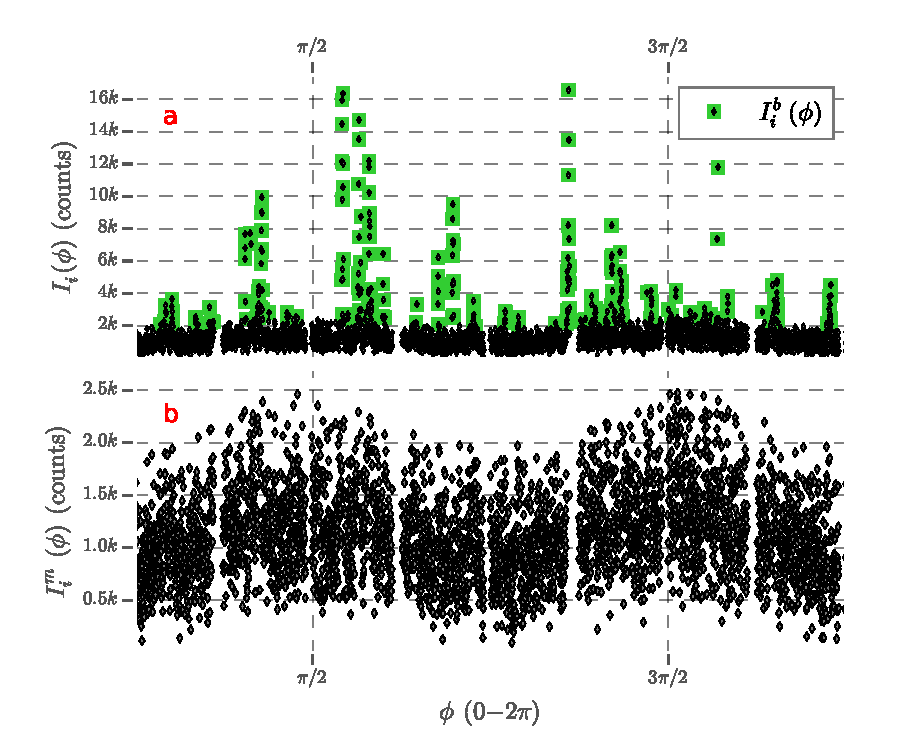
\includegraphics[scale=1]{./Fig3Apr7.pdf}
\caption{Separation of bright Bragg spots in the angular intensity profile. \emph{(a)} The $\{111\}$ Bragg ring intensity of a single snapshot exposure $i$. Highlighted in green are the brightest intensities\emph{(b)} Same as \emph{(a)}, but the bright Bragg intensity "spots" are removed, leaving behind the moderate intensity, which form a relatively noisy signal. The angular gaps in \emph{(a)} and \emph{(b)} represent gaps between the detector pixel panels. The variation in counts periodic in $\pi$ is due to beam polarization. Other non-uniformities occur in the analysis, including detector shadows (Supplementary Fig. \ref{supp:prof}). We correlate the the bright and moderate intensities separately (the results are shown in Fig. \ref{fig:Main_result}).}
\label{fig:peaks_rm}
\end{figure}

Prior to correlation, we separated the Bragg ring intensity $I_i(\phi)$ into two components: the brightest Bragg spots (Fig. \ref{fig:peaks_rm}a), and the moderate intensities (Fig. \ref{fig:peaks_rm}b). Specifically we split the intensity according to  

\[
 I^b_i(\phi) =
  \begin{cases} 
      \hfill I_i(\phi)    \hfill &  z_i(\phi) > 2.5 \\
      \hfill 0 \hfill & \text{ otherwise} \\
  \end{cases}
\]

\[
 I^m_i(\phi) =
  \begin{cases} 
      \hfill I_i(\phi)    \hfill &  z_i(\phi) <= 2.5 \\
      \hfill 0 \hfill & \text{ otherwise} \\
  \end{cases}
\]

where $z_i(\phi)$ is a modified standard score in units of the median intensity around the Bragg ring (see Supplemental Section \ref{outlier_filter} for details). 

We averaged $D_{i,j}(\cos \psi)$ separately for the two clusters of intensities to resolve the CXS signals. CXS of the moderate intensities, $D^m_{F}(\phi)$, showed peaks at $\cos \psi = \pm\,  1/3, \pm\, 5/9, \pm\, 7/9$ indicating the presence of twinning (Fig. \ref{fig:Main_result}c). On the other hand, the CXS of the bright Bragg spots, $D^b_{F}(\phi)$, only showed peaks at $\cos \psi = \pm 1/3$ (Fig. \ref{fig:Main_result}d), implying that the domains which scattered the brightest Bragg spots were not twinned.

\begin{figure}[H]
\centering
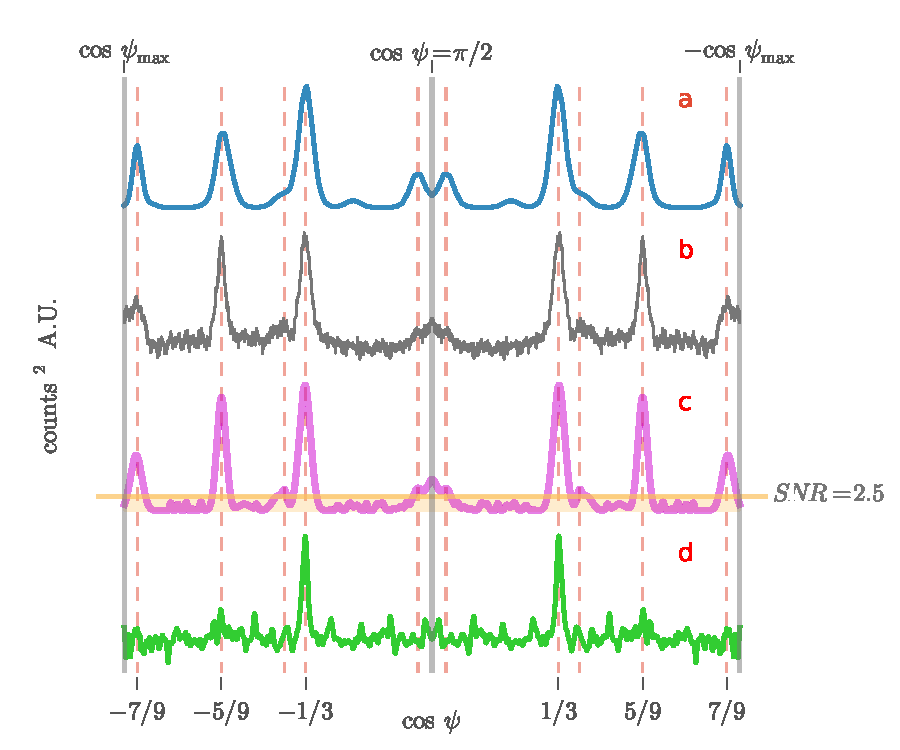
\includegraphics[scale=1]{./Fig4Apr8.pdf}
\caption{Simulated and measured CXS for the $\{111\}$ Bragg ring. \emph{(a)} Simulated CXS for the gold decahedron in Fig. \ref{fig:contrast}b. \emph{(b)} The mirror-symmetric difference correlation of the moderate intensities, $D^m_F(\cos \psi)$, which imposes Friedel symmetry (Supplementary Section \ref{supp:Friedel}) This data represents an average of $1.6\cdot 10^5$ exposures. \emph{(c)} The Gaussian fit $G(\cos \psi)$ (Supplementary Section \ref{supp:Gauss}), fit directly to $D^m_F(\cos \psi)$. The horizontal line marks an SNR (Supplementary Section \ref{supp:Z}) value of 2.5. There are many small peaks with low SNR which are likely noise. \emph{(d)} The mirror-symmetric difference correlation of the bright Bragg intensities, $D^b_F(\cos \psi)$. The absence of pronounced peaks at $\cos \psi = \pm 5/9 , \pm 7/9$ indicates that this signal arises from a population of non-twinned scattering domains. Also, the relatively sharp width of the CXS peaks at $\cos \psi = \pm 1/3$ indicates that the corresponding NP domains are larger than the twinned domains which produced the CXS shown in \emph{(b)}.  Dashed vertical lines (red) are predicted CXS signal from the NNT model, as well as other significant CXS signals. }
\label{fig:Main_result}
\end{figure}

Similar to how the width of a Bragg spot (peak) relates to the corresponding NP domain size, the width of the CXS peak can be used to infer the size of the NP domains which scattered correlated photons (Supplemental Section \ref{widths_small}). We examine the full-width-half-max (FWHM) of the CXS peaks at $\cos \psi = 1/3$ for both data clusters and find that the peak in $D^m_F{\cos \psi}$ has a FWHM of \SI{0.036}{\radian}, while the peak in $D^b_F{\cos \psi}$ has a FWHM of \SI{0.019}{\radian} (Supplemental Section \ref{widths_large}). Because the peak width is inversely proportional to the domain size  (Supplemental Section \ref{widths_small}), we infer that the bright Bragg spots come from larger NP domains within the population. For size estimates of the NP domains within the sample, see Supplemental Sections \ref{widths_small} and \ref{widths_large}.

Figure \ref{fig:pk} shows the signal-to-noise ratio (SNR) scaling for significant CXS peaks in $D^m_F(\cos \psi)$. As expected \cite{kirian2011signal}, the signal to noise increases with the square root of $N$. An SNR of $2.5$ is obtained after averaging $N=1000,\,1800,\,7200,$ and $\,85000$ snapshot exposures for peaks at $\cos \psi = \pm 1/3,\, \pm 5/9,\, \pm 7/9,$ and $\pm 0.4$, respectively.

While the NNT model only predicts peaks at $\cos \psi = \pm1/3, \pm 5/9, \pm 7/9$, additional peaks with an $SNR > 2.5$ are also present (Figs. \ref{fig:Main_result}, \ref{fig:pk}) that may indicate more complicated MTP structure. Each measured CXS peak represents a potential constraint on atomic models, and these additional peaks could be used to refine more complicated twinning patterns. The ability of CXS to identify complex atomic scale structures in ensembles of nanoparticles has potential for a wide range of applications. 
 
\begin{figure}[H]
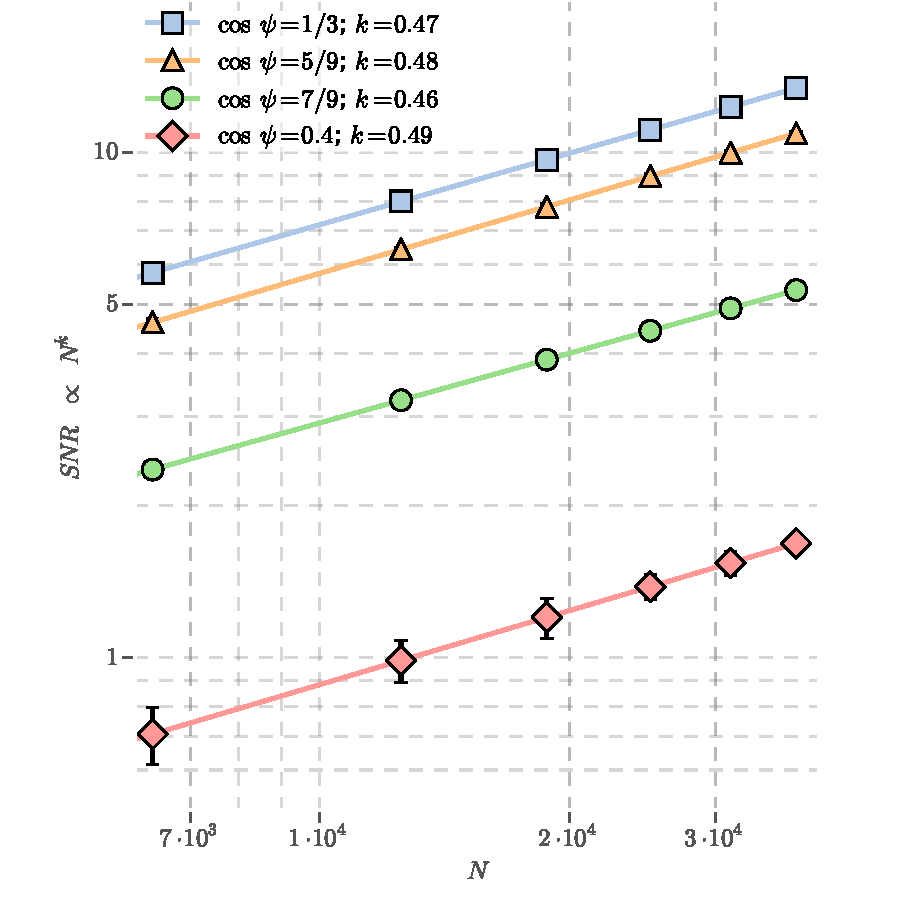
\includegraphics[scale=0.6]{./Fig5Apr8.pdf}
\caption{The estimated SNR of 4 significant CXS peaks in $D^m_F(\cos \psi)$ as a function of $N$, the number of averaged snapshot exposures. The SNR is defined in Supplementary Section \ref{supp:Z}.}
\label{fig:pk}
\end{figure}

\section{Summary}
We have demonstrated the power of the CXS technique to obtain structural details of a large ensemble of similar objects at a resolution which can be used to compare with atomic models. Our analysis allowed us to separate our sample into two populations, smaller, twinned NP domains, and larger, non-twinned NP domains. From the statistics of observed features in the CXS of the small, twinned domains, we assessed the confidence level of the different observed correlated scattering features. We found remarkable agreement with an atomic twinning model, and we also resolved additional CXS signals which could be used for model refinement. Advances in X-ray instrumentation and sources have reached a critical point from which CXS has become feasible \cite{emma2010first, ishikawa2012compact}. Consequently, the technique itself is in its infancy. The true power in a CXS measurement is in the richness of its information. Here we only reported on the measurement of intensity correlations at a single scattering vector, namely $q_{111}$ for gold FCC NPs, yet even more information is contained in the cross correlations and auto correlations of all measured scattering angles. As sample injection and data collection tools continue to improve, so should the ability to refine the angular intensity correlation functions hidden within snapshot X-ray measurements, providing a means for better model fitting and a better understanding of some of nature's smallest structures.

\section{Methods}
Gold NPs (specified to be \SI{60}{\nm} in diameter) were purchased from Nanopartz Inc. (Loveland, CO, USA) and suspended in LCP (lipid cubic phase) \cite{ai2000membrane, cheng1998simple, caffrey2009crystallizing, misquitta2003detergents} at a concentration of \SI{40}{\mg \per \ml}. The viscous LCP solution was injected into the beam as a constant stream using a Hamilton 7780-01 syringe needle with inner diameter \SI{130}{\micro \meter}. The SACLA beam was focused down to a roughly \SI{1.5x2.4}{\micro \meter} spot size. We estimate at least $9.8\cdot10^3$ NPs per each exposed volume (Supplementary Section \ref{number_of_NPs}). Prior to calculating the CXS, we detected and separated the bright Bragg spots (peaks) from the moderate intensities. By correlating the moderate intensities, we demonstrate the ability of CXS to extract signal from snapshots that appear at first glance to be complete noise (Fig. \ref{fig:peaks_rm}b).

For the analysis we worked solely with the $\{111\}$ Bragg ring. The beam repetition rate was 30 Hz. The pulses were measured using an MPCCD 8-panel detector in a wide-angle setup, with a beam energy of \SI{8.6}{\kilo \electronvolt} and a maximum momentum transfer of $3.4 \, \angstrom^{-1}$ ($\lambda = $ \SI{1.442}{\angstrom}). The scattering angle $\theta_{111}$ was \SI{17.83}{\degree} and for $\{111\}$ auto-correlationsz ($\theta_1 = \theta_2 = \theta_{111}$ in equation (\ref{psimax})), $\psi_{\max}$ was \SI{144.3}{\degree}. With this setup we acquired roughly $5 \cdot 10^5$ snapshot exposures of gold NPs. 

The goal of the analysis was to determine the angles $\psi$ which show angular intensity correlations at the $\{111\}$ Bragg ring, and to compare the results with the values in $\bm {\Psi}_{111}$ and $\bm \Psi^{A,B}_{111}$.

As previously reported, straightforward computation of equation (\ref{corz}) is dominated by artifactual correlations associated with the experiment \cite{mendez2014observation}. Examples of these correlations include pixel cross-talk, detector shadows, and scattering anisotropies due to an inhomogeneous sample.  Assuming different exposures will have similar artifactual asymmetries,  equation (\ref{difcorz}) will suppress any asymmetries via subtraction, thus minimizing any artifactual correlation signal.

\section*{Acknowledgements}
The XFEL experiments were performed at the BL3 of SACLA with the approval of the Japan Synchrotron Radiation Research Institute (JASRI) (Proposal No. 2013B8009)
SD thanks  John Spence and Gordon J. Brown Jr for their advice and encouragement.

%\bibliographystyle{naturemag}
%\bibliography{myreferences}

\begin{thebibliography}{10}
\expandafter\ifx\csname url\endcsname\relax
  \def\url#1{\texttt{#1}}\fi
\expandafter\ifx\csname urlprefix\endcsname\relax\def\urlprefix{URL }\fi
\providecommand{\bibinfo}[2]{#2}
\providecommand{\eprint}[2][]{\url{#2}}

\bibitem{kam1977determination}
\bibinfo{author}{Kam, Z.}
\newblock \bibinfo{title}{Determination of macromolecular structure in solution
  by spatial correlation of scattering fluctuations}.
\newblock \emph{\bibinfo{journal}{Macromolecules}}
  \textbf{\bibinfo{volume}{10}}, \bibinfo{pages}{927--934}
  (\bibinfo{year}{1977}).

\bibitem{saldin2010beyond}
\bibinfo{author}{Saldin, D.} \emph{et~al.}
\newblock \bibinfo{title}{Beyond small-angle x-ray scattering: Exploiting
  angular correlations}.
\newblock \emph{\bibinfo{journal}{Physical Review B}}
  \textbf{\bibinfo{volume}{81}}, \bibinfo{pages}{174105}
  (\bibinfo{year}{2010}).

\bibitem{saldin2009structure}
\bibinfo{author}{Saldin, D.}, \bibinfo{author}{Shneerson, V.},
  \bibinfo{author}{Fung, R.} \& \bibinfo{author}{Ourmazd, A.}
\newblock \bibinfo{title}{Structure of isolated biomolecules obtained from
  ultrashort x-ray pulses: exploiting the symmetry of random orientations}.
\newblock \emph{\bibinfo{journal}{Journal of Physics: Condensed Matter}}
  \textbf{\bibinfo{volume}{21}}, \bibinfo{pages}{134014}
  (\bibinfo{year}{2009}).

\bibitem{saldin2010structure}
\bibinfo{author}{Saldin, D.} \emph{et~al.}
\newblock \bibinfo{title}{Structure of a single particle from scattering by
  many particles randomly oriented about an axis: toward structure solution
  without crystallization?}
\newblock \emph{\bibinfo{journal}{New Journal of Physics}}
  \textbf{\bibinfo{volume}{12}}, \bibinfo{pages}{035014}
  (\bibinfo{year}{2010}).

\bibitem{pande2014deducing}
\bibinfo{author}{Pande, K.}, \bibinfo{author}{Schwander, P.},
  \bibinfo{author}{Schmidt, M.} \& \bibinfo{author}{Saldin, D.}
\newblock \bibinfo{title}{Deducing fast electron density changes in randomly
  orientated uncrystallized biomolecules in a pump--probe experiment}.
\newblock \emph{\bibinfo{journal}{Philosophical Transactions of the Royal
  Society of London B: Biological Sciences}} \textbf{\bibinfo{volume}{369}},
  \bibinfo{pages}{20130332} (\bibinfo{year}{2014}).

\bibitem{schenk2015potential}
\bibinfo{author}{Schenk, G.}, \bibinfo{author}{Krajina, B.},
  \bibinfo{author}{Spakowitz, A.} \& \bibinfo{author}{Doniach, S.}
\newblock \bibinfo{title}{Potential for measurement of the distribution of dna
  folds in complex environments using correlated x-ray scattering}.
\newblock \emph{\bibinfo{journal}{Modern Physics Letters B}}
  \bibinfo{pages}{1650117} (\bibinfo{year}{2015}).

\bibitem{liu2013three}
\bibinfo{author}{Liu, H.}, \bibinfo{author}{Poon, B.~K.},
  \bibinfo{author}{Saldin, D.~K.}, \bibinfo{author}{Spence, J.~C.} \&
  \bibinfo{author}{Zwart, P.~H.}
\newblock \bibinfo{title}{Three-dimensional single-particle imaging using
  angular correlations from x-ray laser data}.
\newblock \emph{\bibinfo{journal}{Acta Crystallographica Section A: Foundations
  of Crystallography}} \textbf{\bibinfo{volume}{69}}, \bibinfo{pages}{365--373}
  (\bibinfo{year}{2013}).

\bibitem{chen2012structure}
\bibinfo{author}{Chen, G.} \emph{et~al.}
\newblock \bibinfo{title}{Structure determination of pt-coated au dumbbells via
  fluctuation x-ray scattering}.
\newblock \emph{\bibinfo{journal}{Journal of synchrotron radiation}}
  \textbf{\bibinfo{volume}{19}}, \bibinfo{pages}{695--700}
  (\bibinfo{year}{2012}).

\bibitem{yacaman1981effect}
\bibinfo{author}{Yacam{\'a}n, M.}, \bibinfo{author}{Fuentes, S.} \&
  \bibinfo{author}{Dominguez, J.}
\newblock \bibinfo{title}{The effect of shape and crystal structure of small
  particles on their catalytic activity}.
\newblock \emph{\bibinfo{journal}{Surface Science}}
  \textbf{\bibinfo{volume}{106}}, \bibinfo{pages}{472 -- 477}
  (\bibinfo{year}{1981}).
  
\bibitem{narayanan2005catalysis}
\bibinfo{author}{Narayanan, R.} \& \bibinfo{author}{El-Sayed, M.~A.}
\newblock \bibinfo{title}{Catalysis with transition metal nanoparticles in
  colloidal solution: nanoparticle shape dependence and stability}.
\newblock \emph{\bibinfo{journal}{The Journal of Physical Chemistry B}}
  \textbf{\bibinfo{volume}{109}}, \bibinfo{pages}{12663--12676}
  (\bibinfo{year}{2005}).

\bibitem{narayanan2004shape}
\bibinfo{author}{Narayanan, R.} \& \bibinfo{author}{El-Sayed, M.~A.}
\newblock \bibinfo{title}{Shape-dependent catalytic activity of platinum
  nanoparticles in colloidal solution}.
\newblock \emph{\bibinfo{journal}{Nano letters}} \textbf{\bibinfo{volume}{4}},
  \bibinfo{pages}{1343--1348} (\bibinfo{year}{2004}).

\bibitem{ino1969stability}
\bibinfo{author}{Ino, S.}
\newblock \bibinfo{title}{Stability of multiply-twinned particles}.
\newblock \emph{\bibinfo{journal}{Journal of the Physical Society of Japan}}
  \textbf{\bibinfo{volume}{27}}, \bibinfo{pages}{941--953}
  (\bibinfo{year}{1969}).

\bibitem{marks1983modified}
\bibinfo{author}{Marks, L.}
\newblock \bibinfo{title}{Modified wulff constructions for twinned particles}.
\newblock \emph{\bibinfo{journal}{Journal of Crystal Growth}}
  \textbf{\bibinfo{volume}{61}}, \bibinfo{pages}{556--566}
  (\bibinfo{year}{1983}).

\bibitem{howie1984elastic}
\bibinfo{author}{Howie, A.} \& \bibinfo{author}{Marks, L.}
\newblock \bibinfo{title}{Elastic strains and the energy balance for multiply
  twinned particles}.
\newblock \emph{\bibinfo{journal}{Philosophical Magazine A}}
  \textbf{\bibinfo{volume}{49}}, \bibinfo{pages}{95--109}
  (\bibinfo{year}{1984}).

\bibitem{marks1984surface}
\bibinfo{author}{Marks, L.}
\newblock \bibinfo{title}{Surface structure and energetics of multiply twinned
  particles}.
\newblock \emph{\bibinfo{journal}{Philosophical Magazine A}}
  \textbf{\bibinfo{volume}{49}}, \bibinfo{pages}{81--93}
  (\bibinfo{year}{1984}).

\bibitem{ringe2013kinetic}
\bibinfo{author}{Ringe, E.}, \bibinfo{author}{Van~Duyne, R.~P.} \&
  \bibinfo{author}{Marks, L.~D.}
\newblock \bibinfo{title}{Kinetic and thermodynamic modified wulff
  constructions for twinned nanoparticles}.
\newblock \emph{\bibinfo{journal}{The Journal of Physical Chemistry C}}
  \textbf{\bibinfo{volume}{117}}, \bibinfo{pages}{15859--15870}
  (\bibinfo{year}{2013}).

\bibitem{heinemann1979structure}
\bibinfo{author}{Heinemann, K.}, \bibinfo{author}{Yacaman, M.},
  \bibinfo{author}{Yang, C.} \& \bibinfo{author}{Poppa, H.}
\newblock \bibinfo{title}{The structure of small, vapor-deposited particles: I.
  experimental study of single crystals and particles with pentagonal
  profiles}.
\newblock \emph{\bibinfo{journal}{Journal of Crystal Growth}}
  \textbf{\bibinfo{volume}{47}}, \bibinfo{pages}{177--186}
  (\bibinfo{year}{1979}).

\bibitem{yacaman1979structure}
\bibinfo{author}{Yacaman, M.}, \bibinfo{author}{Heinemann, K.},
  \bibinfo{author}{Yang, C.} \& \bibinfo{author}{Poppa, H.}
\newblock \bibinfo{title}{The structure of small, vapor-deposited particles:
  II. experimental study of particles with hexagonal profile}.
\newblock \emph{\bibinfo{journal}{Journal of Crystal Growth}}
  \textbf{\bibinfo{volume}{47}}, \bibinfo{pages}{187--195}
  (\bibinfo{year}{1979}).

\bibitem{langille2012stepwise}
\bibinfo{author}{Langille, M.~R.}, \bibinfo{author}{Zhang, J.},
  \bibinfo{author}{Personick, M.~L.}, \bibinfo{author}{Li, S.} \&
  \bibinfo{author}{Mirkin, C.~A.}
\newblock \bibinfo{title}{Stepwise evolution of spherical seeds into 20-fold
  twinned icosahedra}.
\newblock \emph{\bibinfo{journal}{Science}} \textbf{\bibinfo{volume}{337}},
  \bibinfo{pages}{954--957} (\bibinfo{year}{2012}).

\bibitem{yang1979crystallography}
\bibinfo{author}{Yang, C.}
\newblock \bibinfo{title}{Crystallography of decahedral and icosahedral
  particles: I. geometry of twinning}.
\newblock \emph{\bibinfo{journal}{Journal of Crystal Growth}}
  \textbf{\bibinfo{volume}{47}}, \bibinfo{pages}{274--282}
  (\bibinfo{year}{1979}).

\bibitem{yang1979crystallography2}
\bibinfo{author}{Yang, C.}, \bibinfo{author}{Yacaman, M.} \&
  \bibinfo{author}{Heinemann, K.}
\newblock \bibinfo{title}{Crystallography of decahedral and icosahedral
  particles: Ii. high symmetry orientations}.
\newblock \emph{\bibinfo{journal}{Journal of Crystal Growth}}
  \textbf{\bibinfo{volume}{47}}, \bibinfo{pages}{283--290}
  (\bibinfo{year}{1979}).

\bibitem{dai2002shapes}
\bibinfo{author}{Dai, Z.~R.}, \bibinfo{author}{Sun, S.} \&
  \bibinfo{author}{Wang, Z.~L.}
\newblock \bibinfo{title}{Shapes, multiple twins and surface structures of
  monodisperse fept magnetic nanocrystals}.
\newblock \emph{\bibinfo{journal}{Surface science}}
  \textbf{\bibinfo{volume}{505}}, \bibinfo{pages}{325--335}
  (\bibinfo{year}{2002}).

\bibitem{marks1981high}
\bibinfo{author}{Marks, L.} \& \bibinfo{author}{Smith, D.~J.}
\newblock \bibinfo{title}{High resolution studies of small particles of gold
  and silver: I. multiply-twinned particles}.
\newblock \emph{\bibinfo{journal}{Journal of Crystal Growth}}
  \textbf{\bibinfo{volume}{54}}, \bibinfo{pages}{425--432}
  (\bibinfo{year}{1981}).

\bibitem{yacaman1992electron}
\bibinfo{author}{Jos{\'e}-Yacam{\'a}n, M.} \& \bibinfo{author}{Avalos-Borja,
  M.}
\newblock \bibinfo{title}{Electron microscopy of metallic nano particles using
  high-and medium-resolution techniques}.
\newblock \emph{\bibinfo{journal}{Catalysis Reviews}}
  \textbf{\bibinfo{volume}{34}}, \bibinfo{pages}{55--127}
  (\bibinfo{year}{1992}).

\bibitem{chen2013three}
\bibinfo{author}{Chen, C.-C.} \emph{et~al.}
\newblock \bibinfo{title}{Three-dimensional imaging of dislocations in a
  nanoparticle at atomic resolution}.
\newblock \emph{\bibinfo{journal}{Nature}} \textbf{\bibinfo{volume}{496}},
  \bibinfo{pages}{74--77} (\bibinfo{year}{2013}).

\bibitem{kurta2013xray}
\bibinfo{author}{Kurta", R.~P.}
\newblock \bibinfo{title}{X-ray cross-correlation analysis of liquid crystal
  membranes in the vicinity of the hexatic-smectic phase transition}.
\newblock \emph{\bibinfo{journal}{Physical Review E}}
  \textbf{\bibinfo{volume}{88}} (\bibinfo{year}{2013}).

\bibitem{schroer2014characteristics}
\bibinfo{author}{Schroer, M.}, \bibinfo{author}{Gutt, C.} \&
  \bibinfo{author}{Gr{\"u}bel, G.}
\newblock \bibinfo{title}{Characteristics of angular cross correlations studied
  by light scattering from two-dimensional microsphere films}.
\newblock \emph{\bibinfo{journal}{Physical Review E}}
  \textbf{\bibinfo{volume}{90}}, \bibinfo{pages}{012309}
  (\bibinfo{year}{2014}).

\bibitem{lehmkuhler2014detecting}
\bibinfo{author}{Lehmk{\"u}hler, F.}, \bibinfo{author}{Gr{\"u}bel, G.} \&
  \bibinfo{author}{Gutt, C.}
\newblock \bibinfo{title}{Detecting orientational order in model systems by
  x-ray cross-correlation methods}.
\newblock \emph{\bibinfo{journal}{Journal of applied crystallography}}
  \textbf{\bibinfo{volume}{47}}, \bibinfo{pages}{1315--1323}
  (\bibinfo{year}{2014}).

\bibitem{kurta2012xray}
\bibinfo{author}{Kurta, R.}, \bibinfo{author}{Altarelli, M.},
  \bibinfo{author}{Weckert, E.} \& \bibinfo{author}{Vartanyants, I.}
\newblock \bibinfo{title}{X-ray cross-correlation analysis applied to
  disordered two-dimensional systems}.
\newblock \emph{\bibinfo{journal}{Physical Review B}}
  \textbf{\bibinfo{volume}{85}}, \bibinfo{pages}{184204}
  (\bibinfo{year}{2012}).

\bibitem{pedrini2013two}
\bibinfo{author}{Pedrini, B.} \emph{et~al.}
\newblock \bibinfo{title}{Two-dimensional structure from random multiparticle
  x-ray scattering images using cross-correlations}.
\newblock \emph{\bibinfo{journal}{Nature communications}}
  \textbf{\bibinfo{volume}{4}}, \bibinfo{pages}{1647} (\bibinfo{year}{2013}).

\bibitem{saldin2011new}
\bibinfo{author}{Saldin, D.} \emph{et~al.}
\newblock \bibinfo{title}{New light on disordered ensembles: ab initio
  structure determination of one particle from scattering fluctuations of many
  copies}.
\newblock \emph{\bibinfo{journal}{Physical Review Letters}}
  \textbf{\bibinfo{volume}{106}}, \bibinfo{pages}{115501}
  (\bibinfo{year}{2011}).

\bibitem{elser2011strategies}
\bibinfo{author}{Elser, V.}
\newblock \bibinfo{title}{Strategies for processing diffraction data from
  randomly oriented particles}.
\newblock \emph{\bibinfo{journal}{Ultramicroscopy}}
  \textbf{\bibinfo{volume}{111}}, \bibinfo{pages}{788--792}
  (\bibinfo{year}{2011}).

\bibitem{kam1980reconstruction}
\bibinfo{author}{Kam, Z.}
\newblock \bibinfo{title}{The reconstruction of structure from electron
  micrographs of randomly oriented particles}.
\newblock \emph{\bibinfo{journal}{Journal of theoretical biology}}
  \textbf{\bibinfo{volume}{82}}, \bibinfo{pages}{15--39}
  (\bibinfo{year}{1980}).

\bibitem{poon2015use}
\bibinfo{author}{Poon, H.} \& \bibinfo{author}{Saldin, D.}
\newblock \bibinfo{title}{Use of triple correlations for the sign
  determinations of expansion coefficients of symmetric approximations to the
  diffraction volumes of regular viruses}.
\newblock \emph{\bibinfo{journal}{Structural Dynamics}}
  \textbf{\bibinfo{volume}{2}}, \bibinfo{pages}{041716} (\bibinfo{year}{2015}).

\bibitem{starodub2012single}
\bibinfo{author}{Starodub, D.} \emph{et~al.}
\newblock \bibinfo{title}{Single-particle structure determination by
  correlations of snapshot x-ray diffraction patterns}.
\newblock \emph{\bibinfo{journal}{Nature communications}}
  \textbf{\bibinfo{volume}{3}}, \bibinfo{pages}{1276} (\bibinfo{year}{2012}).

\bibitem{saldin2011reconstructing}
\bibinfo{author}{Saldin, D.}, \bibinfo{author}{Poon, H.-C.},
  \bibinfo{author}{Schwander, P.}, \bibinfo{author}{Uddin, M.} \&
  \bibinfo{author}{Schmidt, M.}
\newblock \bibinfo{title}{Reconstructing an icosahedral virus from
  single-particle diffraction experiments}.
\newblock \emph{\bibinfo{journal}{Optics express}}
  \textbf{\bibinfo{volume}{19}}, \bibinfo{pages}{17318--17335}
  (\bibinfo{year}{2011}).

\bibitem{wochner2009x}
\bibinfo{author}{Wochner, P.} \emph{et~al.}
\newblock \bibinfo{title}{X-ray cross correlation analysis uncovers hidden
  local symmetries in disordered matter}.
\newblock \emph{\bibinfo{journal}{Proceedings of the National Academy of
  Sciences}} \textbf{\bibinfo{volume}{106}}, \bibinfo{pages}{11511--11514}
  (\bibinfo{year}{2009}).

\bibitem{altarelli2010x}
\bibinfo{author}{Altarelli, M.}, \bibinfo{author}{Kurta, R.} \&
  \bibinfo{author}{Vartanyants, I.}
\newblock \bibinfo{title}{X-ray cross-correlation analysis and local symmetries
  of disordered systems: General theory}.
\newblock \emph{\bibinfo{journal}{Physical Review B}}
  \textbf{\bibinfo{volume}{82}}, \bibinfo{pages}{104207}
  (\bibinfo{year}{2010}).

\bibitem{kurta2013cross}
\bibinfo{author}{Kurta, R.}, \bibinfo{author}{Chesnokov, Y.},
  \bibinfo{author}{Weckert, E.} \& \bibinfo{author}{Vartanyants, I.}
\newblock \bibinfo{title}{Cross-correlation analysis of x-ray scattering from
  oxygen clusters}.
\newblock In \emph{\bibinfo{booktitle}{Journal of Physics: Conference Series}},
  vol. \bibinfo{volume}{463}, \bibinfo{pages}{012046}
  (\bibinfo{organization}{IOP Publishing}, \bibinfo{year}{2013}).

\bibitem{malmerberg2015operational}
\bibinfo{author}{Malmerberg, E.}, \bibinfo{author}{Kerfeld, C.~A.} \&
  \bibinfo{author}{Zwart, P.~H.}
\newblock \bibinfo{title}{Operational properties of fluctuation x-ray
  scattering data}.
\newblock \emph{\bibinfo{journal}{IUCrJ}} \textbf{\bibinfo{volume}{2}},
  \bibinfo{pages}{309--316} (\bibinfo{year}{2015}).

\bibitem{pande2015simulations}
\bibinfo{author}{Pande, K.}, \bibinfo{author}{Schmidt, M.},
  \bibinfo{author}{Schwander, P.} \& \bibinfo{author}{Saldin, D.}
\newblock \bibinfo{title}{Simulations on time-resolved structure determination
  of uncrystallized biomolecules in the presence of shot noise}.
\newblock \emph{\bibinfo{journal}{Structural Dynamics}}
  \textbf{\bibinfo{volume}{2}}, \bibinfo{pages}{024103} (\bibinfo{year}{2015}).

\bibitem{liu2012computation}
\bibinfo{author}{Liu, H.}, \bibinfo{author}{Poon, B.~K.},
  \bibinfo{author}{Janssen, A.~J.} \& \bibinfo{author}{Zwart, P.~H.}
\newblock \bibinfo{title}{Computation of fluctuation scattering profiles via
  three-dimensional zernike polynomials}.
\newblock \emph{\bibinfo{journal}{Acta Crystallographica Section A: Foundations
  of Crystallography}} \textbf{\bibinfo{volume}{68}}, \bibinfo{pages}{561--567}
  (\bibinfo{year}{2012}).

\bibitem{mendez2014observation}
\bibinfo{author}{Mendez, D.} \emph{et~al.}
\newblock \bibinfo{title}{Observation of correlated x-ray scattering at atomic
  resolution}.
\newblock \emph{\bibinfo{journal}{Phil. Trans. R. Soc. B}}
  \textbf{\bibinfo{volume}{369}}, \bibinfo{pages}{20130315}
  (\bibinfo{year}{2014}).

\bibitem{kirian2011signal}
\bibinfo{author}{Kirian, R.~A.}, \bibinfo{author}{Schmidt, K.~E.},
  \bibinfo{author}{Wang, X.}, \bibinfo{author}{Doak, R.~B.} \&
  \bibinfo{author}{Spence, J.~C.}
\newblock \bibinfo{title}{Signal, noise, and resolution in correlated
  fluctuations from snapshot small-angle x-ray scattering}.
\newblock \emph{\bibinfo{journal}{Physical Review E}}
  \textbf{\bibinfo{volume}{84}}, \bibinfo{pages}{011921}
  (\bibinfo{year}{2011}).

\bibitem{neutze2000potential}
\bibinfo{author}{Neutze, R.}, \bibinfo{author}{Wouts, R.},
  \bibinfo{author}{van~der Spoel, D.}, \bibinfo{author}{Weckert, E.} \&
  \bibinfo{author}{Hajdu, J.}
\newblock \bibinfo{title}{Potential for biomolecular imaging with femtosecond
  x-ray pulses}.
\newblock \emph{\bibinfo{journal}{Nature}} \textbf{\bibinfo{volume}{406}},
  \bibinfo{pages}{752--757} (\bibinfo{year}{2000}).

\bibitem{kam1981fluctuation}
\bibinfo{author}{Kam, Z.}, \bibinfo{author}{Koch, M.} \&
  \bibinfo{author}{Bordas, J.}
\newblock \bibinfo{title}{Fluctuation x-ray scattering from biological
  particles in frozen solution by using synchrotron radiation}.
\newblock \emph{\bibinfo{journal}{Proceedings of the National Academy of
  Sciences}} \textbf{\bibinfo{volume}{78}}, \bibinfo{pages}{3559--3562}
  (\bibinfo{year}{1981}).

\bibitem{misquitta2003detergents}
\bibinfo{author}{Misquitta, Y.} \& \bibinfo{author}{Caffrey, M.}
\newblock \bibinfo{title}{Detergents destabilize the cubic phase of monoolein:
  implications for membrane protein crystallization}.
\newblock \emph{\bibinfo{journal}{Biophysical journal}}
  \textbf{\bibinfo{volume}{85}}, \bibinfo{pages}{3084--3096}
  (\bibinfo{year}{2003}).

\bibitem{ai2000membrane}
\bibinfo{author}{Ai, X.} \& \bibinfo{author}{Caffrey, M.}
\newblock \bibinfo{title}{Membrane protein crystallization in lipidic
  mesophases: detergent effects}.
\newblock \emph{\bibinfo{journal}{Biophysical journal}}
  \textbf{\bibinfo{volume}{79}}, \bibinfo{pages}{394--405}
  (\bibinfo{year}{2000}).

\bibitem{cheng1998simple}
\bibinfo{author}{Cheng, A.}, \bibinfo{author}{Hummel, B.},
  \bibinfo{author}{Qiu, H.} \& \bibinfo{author}{Caffrey, M.}
\newblock \bibinfo{title}{A simple mechanical mixer for small viscous
  lipid-containing samples}.
\newblock \emph{\bibinfo{journal}{Chemistry and Physics of Lipids}}
  \textbf{\bibinfo{volume}{95}}, \bibinfo{pages}{11--21}
  (\bibinfo{year}{1998}).

\bibitem{caffrey2009crystallizing}
\bibinfo{author}{Caffrey, M.} \& \bibinfo{author}{Cherezov, V.}
\newblock \bibinfo{title}{Crystallizing membrane proteins using lipidic
  mesophases}.
\newblock \emph{\bibinfo{journal}{Nature protocols}}
  \textbf{\bibinfo{volume}{4}}, \bibinfo{pages}{706--731}
  (\bibinfo{year}{2009}).

\bibitem{emma2010first}
\bibinfo{author}{Emma, P.} \emph{et~al.}
\newblock \bibinfo{title}{First lasing and operation of an
  {\aa}ngstrom-wavelength free-electron laser}.
\newblock \emph{\bibinfo{journal}{nature photonics}}
  \textbf{\bibinfo{volume}{4}}, \bibinfo{pages}{641--647}
  (\bibinfo{year}{2010}).

\bibitem{ishikawa2012compact}
\bibinfo{author}{Ishikawa, T.} \emph{et~al.}
\newblock \bibinfo{title}{A compact x-ray free-electron laser emitting in the
  sub-angstrom region}.
\newblock \emph{\bibinfo{journal}{Nature Photonics}}
  \textbf{\bibinfo{volume}{6}}, \bibinfo{pages}{540--544}
  (\bibinfo{year}{2012}).

\end{thebibliography}


%%%%%%%%%%%
% SUPPLEMENTAL%
%%%%%%%%%%%
\newpage


\large{Supplementary Information: Wide-angle correlated X-ray scattering from nanoparticles is consistent with an atomic twinning model}
%\large{Supplementary Information: Wide-angle correlated X-ray scattering from gold nanoparticles demonstrated precise agreement with an atomic twinning model}

\setcounter{equation}{0}
\setcounter{figure}{0}
\setcounter{table}{0}
\setcounter{section}{0}
\setcounter{page}{1}
\makeatletter
\renewcommand{\theequation}{S\arabic{equation}}
\renewcommand{\thefigure}{S\arabic{figure}}
\renewcommand{\thesection}{S\arabic{section}}
%\renewcommand{\bibnumfmt}[1]{[S#1]}
%\renewcommand{\citenumfont}[1]{S#1}

\section{CXS simulation} \label{supp:sim}
We define a solution as a set of identical, non-interacting objects (e.g. molecules) $m$, each with an independent orientation $\bm \omega$ relative to the X-ray beam axis, governed by the objects diffusion constant. We consider $m$ as a collection of $N_a$ atoms each with position vector 
\be
\bm r^m_j (t) = \bm R^m_\omega (t)\cdot \bm r_j + \bm T^m(t) \qquad 1 \le j \le N_a
\ee 
where $\bm R^m_\omega(t)$ is a rotation operator, $\bm T^m (t)$ is a translation operator representing the center of mass position of $m$ at time $t$, and $\bm r_j$ is the position of the $j^{th}$ atom at an arbitrarily defined initial orientation. If we freeze the solution at an instant in time and expose it to X-ray photons of wavelength $\lambda$, then we can measure the scattering factor function

\be
S(\bm q, t) = \left | \sum_m^{N_m} \sum_{j}^{N_a} f_j(q) \,e ^ { -i \,\bm q \cdot \bm  r^m _j (t)  } \right |^2
\ee

Here $f_j(q)$ is the atomic form factor of the $j^{th}$ atom$, \bm q$ represents a position in reciprocal space (e.g. of a pixel) at scattering angle  

\be \label{angle}
\theta= \arcsin \left( \frac{ \lambda \,q}{ 4 \pi} \right )
\ee

and the outer sum is over all $N_m$ exposed objects. In general, $S(\bm q, t)$ may be written as

\be \label{ sums }
S( \bm q, t) = \sum_m^{N_m} \left | A^m_\omega (\bm q ,t ) \right|^2 + \sum _{ m \neq m' } A^m_\omega (\bm q,t ) \left (A^{m'}_\omega (\bm q,t ) \right )^*
\ee

where 

\be
A^m_\omega (\bm q,t ) = \sum_{j}^{N_a} f_j(q) e^{ -i \,\bm q \cdot \bm  r^m_j (t)  }
\ee

The strength of the interference term on the RHS of Supplementary equation (\ref{ sums }) depends on both the concentration of the sample and the magnitude of the momentum transfer vector $q$. For large momentum transfer (wide scattering angles) and/or more dilute samples, the factors $e^{-i \bm q \cdot (  \bm T^m - \bm T^{m'})}$ will approach zero, and we can neglect this term such that we have

\beq \label{ scatter}
S( \bm q, t) &=& \sum_m^{N_m} \left | A^m_\omega (\bm q,t ) \right|^2 \\
&=& \sum_m^{N_m} \left | \sum_{j}^{N_a} f_j(q)\, e^ { -i \,\bm q \cdot \bm  r^m _j (t)} \right | ^2   \\
&=& \sum_m^{N_m} \left | \sum_{j}^{N_a} f_j(q)\, e^ { -i \,\bm q \cdot \left (\bm {R}^m_\omega \left(t\right)\cdot \bm r_j \,+\, \bm {T}^m\left(t\right) \right)} \right | ^2 \\
&=& \sum_m^{N_m} \left | \sum_{j}^{N_a} f_j(q)\, e^ { -i \,\bm q \cdot \bm {R}^m_\omega (t)\cdot \bm r_j }  \right | ^2 
\eeq

Therefore the measured scattering factor for a "dilute" solution is simply a superposition of single molecule scattering factors at various orientations $\bm \omega$.  Instead of considering the precise time dependence of each object (molecule) in solution, however, we consider that, on average, each orientation $\bm \omega$ is occupied by a fixed number of molecules $N_\omega = (N_m/ \int d\omega)$, and that, at each instant, this number is fluctuating by some small amount $\alpha( \bm \omega, t )$ (we are borrowing notation directly from \cite{kam1977determination}). Consider the average isotropic scattering factor over all molecules

\be
S(q) = N _\omega \int S( \bm q, \bm \omega ) d\omega 
\ee

where

\be \label{scattering}
 S(\bm  q, \bm \omega )  = \left | \sum_{j}^{N_a} f_j(q)\, e^ { -i \,\bm q \cdot \bm {R}_\omega \cdot \bm r_j } \right | ^2 
\ee

is the scattering factor of a molecule at orientation $\bm \omega$. Then we can represent $S(\bm q, t)$ as 

\be
S(\bm q, t )  = S ( q )  + \int  S( \bm q, \bm \omega ) \alpha( \bm \omega ,t) d\omega 
\ee

Zvi Kam's main statement is that by measuring 

\be 
\left \langle S(\bm q_1, t )  S(\bm q_2, t )   \right \rangle_t - S( q_1 ) S( q_2 )
\ee

one would resolve a correlation function 

\be
C( \bm q_1, \bm q_2  ) = N_\omega \int S( \bm q_1, \bm \omega ) S( \bm q_2, \bm \omega ) d\omega
\ee

\be \label {kamzcor}
C( q_1, q_2, \cos \psi   ) \propto \int S( \bm q_1, \bm \omega ) S( \bm q_2, \bm \omega ) d\omega
\ee

which depends only on the single particle scattering factor.  The scattering factor in Supplementary equation (\ref{scattering}) is what we simulate, given an arrangement of atoms. We can then easily calculate the expected CXS signal by evaluating the integral in Supplementary equation (\ref{kamzcor}). 

\section{Data analysis stream}
%\begin{figure} [H]
%\includegraphics[]{ana_flow_chart_2.png}
%\label{fig:flow}
%\caption{A schematic showing the flow of data, from the raw data, to the final CXS signal. It is a bit complicated, and we will outline some of the key processes (black boxes) in this supplemental material}
%\end{figure}
The goal of the experiment was to measure Supplementary equation (\ref{kamzcor}) for $q_1 = q_2 = q_{111}$, where $q_{111}$ is the magnitude of the momentum transfer vector at the $\{111\}$ Bragg ring. We did this by measuring the average difference correlation over a set of exposure pairs $\mathcal P$

\begin{equation} \label{supp:c111}
D(\Delta) = \sum_{i,j \in \mathcal P}  \left \langle \,I_{i,j}( \phi) \,I_{i,j}(\phi +\Delta) \right \rangle _\phi
\end{equation}

where $I_{i,j} = \widehat I_i - \widehat I_j$ is the difference of the mean-normalized intensity profiles of two snapshot exposures $i$ and $j$. The full details of the analysis are outlined in the following sections.

\subsection{Convert data}
Scattered photons were recorded on an area detector perpendicular to the forward photon beam. The detector we used was the MPCCD octal sensor, consisting of 8 application-specific integrated circuits (ASICs) which are read out simultaneously, up to 60 Hz. The raw data 

\begin{itemize}
\item are stored on an external user-restricted server, where they remain for one year before being moved to tape storage. 
\item are accessed using in-house SACLA data conversion programs, which output the data as user-accessible hdf5 files.  
\end{itemize}

The in-house software has an option to store reconstructed images, which we employ. The ASICs are assembled into an approximate image, and the relative gains are adjusted. 

Each reconstructed MPCCD image has $2399\times 2399$ pixels. The boundary of each image is padded with zeros (Supplementary Fig. \ref{supp:cart2pol}), so that the reconstructed image size doesn't change if the panels themselves are adjusted between experiments. Each pixel has an integer coordinate $(\,p_x, p_y)$, which also serves as it's array index. We denote the measurement of each pixel during an exposure $s$ as $I_i^{ \mathrm{cart} }(\,p_x\,, \,p_y)$ where ``$\text{cart}$" indicates the image is in cartesian coordinates.


\subsection{Polar interpolation}
Our first task is performing a polar interpolation on the data

\be
I_i^{ \mathrm{cart} }(\,p_x\,, \, p_y) \rightarrow I_i(\,p_r\equiv r \,, p_\phi \equiv \phi)
\ee

for a narrow range of $r \,\in\, [\,r_{\text{low}}\,,\, r_{\text{high}}\,]$ which encompasses the Bragg ring $q_{111}$ (Supplementary Fig. \ref{supp:cart2pol}). This serves to reduce the effective size of the data, which is good for an analysis stream on a large dataset. Loading hundreds of thousands of large images in and out of random-access memory can slow down computation significantly. In this sense, it is better to work with a snippet of each image that we find interesting, which, in this case, is the region near the Bragg ring.

The azimuthal pixel value is given by

\be
\phi = \arctan\left( \frac{p_y - p_b}{p_x - p_a} \right )
\ee

The point $(\,p_a\,,p_b)$ is where the X-ray beam axis intersects the detector. This is the same  as the reciprocal space angle $\phi$ in Supplementary equation (\ref{supp:c111}). We approximate that $(\,p_a\,,p_b)$ remains constant throughout the experiment. One can extrapolate this point of intersection by using the Bragg rings themselves under the assumptions that they are circularly symmetric about the beam axis, and that the detector is perpendicular to the beam axis.

The radial pixel value $r$ is related to the scattering angle $q$ via

\be
r = \frac{d}{\Delta p}\,\,\tan\left(2\,\arcsin \left( \frac{q\,\lambda}{4\,\pi}  \right) \right)
\ee

where $d$, $\Delta p$, and $\lambda$ are the sample-to-detector distance, square pixel length, and photon wavelength, respectively.

With these definitions, we use an elementary floor-nearest-neighbor interpolation to approximate the polar image:

\begin{equation} \label{polimg}
I_i(r \,, \phi) = I_i ^{ \mathrm{cart} }\left ( \lfloor\,  r \,\cos(\phi)+p_a \rfloor, \lfloor\, r\, \sin(\phi) +p_b \rfloor \right)
\end{equation}

where $\lfloor\,\rfloor$ is the floor operation.

\begin{figure}[H]
\includegraphics[]{supp_figs/CART_TO_POLAR.pdf}
\caption{A reconstructed scattering image of gold NPs, and the result of a floor-nearest-neighbor interpolation across the $q_{111}$ Bragg ring. The polar image shown has the same resolution as the cartesian image. There appears to be a shadow on the image, which will lead to artifactual CXS signals.}
\label{supp:cart2pol}
\end{figure}

\subsection{Working with a mask}
Throughout our entire analysis, we work with masked images. We let $M(r\,,\phi)$ represent the polar image mask, a binary image used to exclude the gaps and boundaries surrounding the detector ASICS (panels). Masked pixel values are $0$ and usable pixel values are $1$. Typically there is a mask $M^{\text{cart}}$ for the cartesian images. In this case we would define the polar mask to be $$M(\,r\,, \phi) = M^{\text{cart}} \left ( \lfloor\, r\,\cos(\phi)+p_a \rfloor, \lfloor\,r\, \sin(\phi) +p_b \rfloor \right)$$
Commonly, large scale sensors like these have signal spikes near the edges, so the ASIC edges should be included in the mask. As an example, the mean signal in a masked polar image is defined as

\begin{equation} \label{average_signal}
\overline I_i =  \frac
{\left(\sum\limits_{r\,,\,\phi}\, M( r\,,\phi )\,\,I_i(r\,,\phi) \right) }
 {\left (\sum\limits_{r\,,\,\phi}\, M ( r\,,\phi )\right )}
\end{equation}

For our experiment, we used a fixed mask $M^{\text{cart}}$ and hence $M$ for all images, but these can also vary throughout a given experiment.

%\subsection{Parameterizing the images}
%It is useful in later stages of the analysis to have certain measures for each image. We can use these measures for clustering the data, pairing exposures (which is critical in our analysis, and will be discussed below) and filtering out the images that appear to be corrupted or lacking signal.
%
%From each polar image \ref{polimg} we record several values. These values include obvious measures, such as the mean signal. In addition, however, we would like to store some specialized quantities described below.

\subsection{The 111 Bragg ring position}

\begin{figure}[H]
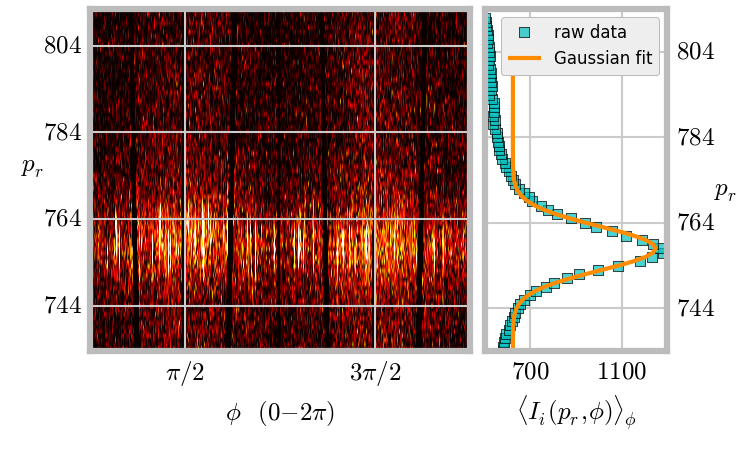
\includegraphics{supp_figs/bragg_ring_position.png}

\caption{Left) A polar image $I_i(r, \phi)$ representing a single snapshot of the gold nanoparticles. Right) The azimuthally averaged intensity and a corresponding Gaussian fit. The center of the Gaussian corresponds to the $\{111\}$ Bragg ring radial position, $r^*_i$}
\end{figure}
In this particular experiment, the sample jet was unstable. Consequently, the sample-to-detector distance fluctuated on a shot by shot basis. In extreme cases, the viscous lipid-cubic-phase solution would kink and clog around the syringe needle tip, causing significant fluctuations in $r^*$ (Supplementary Fig. \ref{supp:p111}).

We will denote the $\{111\}$ Bragg ring radial position snapshot exposure $i$ by $r^*_i$, i.e. the radial pixel ring corresponding to $q_{111}$. Since we do not know the precise sample-to-detector distance of each exposure $s$, we estimate 

\be
r^*_i   \,=\, \text{argmax} \left[ \big \langle I_i \left(\,r\,, \phi\right)\, \big \rangle_{\phi} \right]
\ee

where $\langle \dots \rangle _{\phi}$ denotes the discrete average over $\phi$. Therefore, $r^*_i$ is maximum $r$ across the radial profile of the polar image. Because gold is the only sample component which scatters at these high angles, we assume this is a robust approach.

\begin{figure}[H]
\caption{A histogram of the radial pixel ring corresponding to  $q_{111}$. We predict that the shape of this histogram (with the two peaks near 760 and 772) arises due to fluctuations in the injector system leading to different sample-to-detector positions. One way to fix this would be to use a gas focuses sample injector. Exposure pairing was a critical part of our analysis. We only paired exposures whose $r^*_i$ were in the same radial bin, marked here by the orange vertical lines.}
\includegraphics[]{supp_figs/Fig_p111_supp.pdf}
\label{supp:p111}
\end{figure}

\subsection{The Bragg ring (angular profile) $I_i(\phi)$}
For  the purpose of this paper, we found it sufficient to let 
\be
I_i(\phi) = I_i(r=r^*_i, \phi)
\ee

We sample $\phi$ at $N_{\phi}$ evenly spaced points along the Bragg ring. We fix $N_\phi \ge 2\,\pi\,p_{\text{high}}$. In this way we will sample azimuthally at unit pixel precision at the highest anticipated angles. We let $\varPhi_i$ be the set of all non-masked sampled $\phi$ values in shot $i$:
\be \label{setphi}
\varPhi_i = \left \{ \phi \in   \left \{0\,, \frac{2\,\pi}{N_\phi}\,, \frac{4\,\pi}{N_\phi}\,, \dots \frac{2\,\pi\,(N_\phi-1)}{N_\phi} \right \}\, \big | \,\,M_i(\phi) = 1\right  \}
\ee
where
\be
M_i(\phi) = M \left( \,r=r^*_i \, , \phi \right ) 
\ee
is the corresponding angular intensity mask.
\begin{figure}[H]
\includegraphics[]{supp_figs/Fig_angprof_supp.pdf}
\caption{In blue is the raw calculation of $I_i(\phi)$ for a single snapshot, which shows sharp peaks indicative of larger crystallites. Our motivation is actually to study less crystalline materials in the soft matter regime, so we attempt to remove all signal associated with these larger, more crystalline nanoparticles. The solid yellow line is a biased polynomial, fit to the raw data with the signal spikes (blue x markers). Shown in dashed-black is the unbiased polynomial $y^*_i(\phi)$, fit to the data without the Bragg peaks (red triangle markers).}
\label{supp:prof}
\end{figure}

\subsection{Quantifying angular anisotropies}
As one can see in Supplementary Fig. \ref{supp:prof}, there is a large, slow-varying angular anisotropy in the profile of the Bragg ring $I_i(\phi)$. We seek to suppress any errors this will introduce into the correlation. 

Shadows, beam polarization, and sample inhomogeneity, are but a few sources of systematic noise which can give rise to large angular anisotropies in $I_i(\phi)$. One can see these by eye (Supplementary Figs. \ref{supp:cart2pol}, \ref{supp:prof}). We have a method for overcoming these effects, which depends on the pairing of exposures with similar anisotropies. Here we discuss the quantification of the angular anisotropy.

In order to quantify the anisotropy, we fit 15th degree Chebyshev polynomials of the first kind to the angular intensity profile $I_i(\phi)$. Chebyshev polynomials of the first kind are defined by

\begin{equation}
y(\phi) = c_0\,T_0(\phi) + c_1\,T_1(\phi) + \dots + c_{15} \, T_{15}(\phi) 
\end{equation}

where

\begin{eqnarray}
T_0(\phi) &=& 1 \nonumber\cr
T_1(\phi) &=& x \nonumber \cr
T_{n+1}(\phi) &=& 2\,x\,T_n(\phi) - T_{n-1}(\phi) \nonumber
\end{eqnarray}

The fit is a simple least squares which minimizes the residual

\begin{equation} \label{supp:fit}
E_i =  \sum_{\phi} \big |\, I_i(\phi) - y_i(\phi)\big |^{\,2}
\end{equation}

Note in Supplementary Fig. \ref{supp:prof} the large Bragg spots (peaks). These large signal spikes will bias the residual $E_i$, hence we mask them prior to fitting the polynomial. To detect the signal spikes we use the median outlier filter described in Supplementary Section $\ref{outlier_filter}$. We let $y^*_i$ be the Chebyshev polynomial which minimizes the unbiased residual. Supplementary Fig. \ref{supp:prof} shows two polynomial fits, one to the raw data and another to the data without the Bragg spots. The pairing of exposures according to their angular anisotropies is critical for our analysis, as detailed in the following sections.

\subsection{Exposure pairing} \label{pairing}
For our reported results, we made use of the difference correlation, which involves subtracting pairs of exposures and correlating the residuals. Our data were divided up into $85$ experimental  runs, and each run represented an average of $4500$ usable exposures. We considered a usable exposure to be one where the X-ray shutter was open and the X-ray laser was operating properly (occasionally the laser pulses would cease during a run from complications upstream). We acquired roughly $3.8 \cdot 10^5$ usable exposures, and we did not attempt to compare each exposure with every other exposure. Rather, we only compared and paired exposures that occurred during the same experimental run.

\begin{figure}[H]
\includegraphics[]{supp_figs/shot_mean_histogram.pdf}
\caption{A histogram of the mean intensity of every polar image $I_i(r,\phi)$ across all experimental runs. Only exposures whose mean intensity was greater than 300 units and less than 3000 units were analyzed $(300 \le \overline I_i \le 3000)$.}
\label{fig:shot_mean_histogram}
\end{figure}
%We call the set of all exposures $\{i\}$, and the set of exposures per run $\{i\}_{\mathcal R}$.  
We began by selecting all exposures for analysis according to their total average signal $\overline I_i$ as defined in Supplementary equation (\ref{average_signal}) (Supplementary Fig. \ref{fig:shot_mean_histogram}). We ignored exposures that were too weak $(\overline I_i < 300 \mathrm{\,counts})$ because it is likely that they were recorded when the sample injector failed. Similarly, we rejected exposures that were too strong $(\overline I_i > 3000 \mathrm{\,counts})$, for they may include non-liner effects on the detector such as faulty pixel responses.

After filtering based on mean intensity, exposures within a certain run were grouped according to their respective $r^*_i$. Each exposure $i$ was assigned to a subgroup based on the floored value $\lfloor r^*_i \rfloor$, i.e. the closest integer less than $r^*_i$ (the vertical orange lines in Supplementary Fig. \ref{supp:p111} represent the group bins). Pairs were constrained to be formed using exposures from the same subgroup. The pairing process involved an optimization step in which exposures were recursively compared to each other; forming subgroups for pairing serves to reduce the required computation time. 

\emph{We required that an exposure can only be used once during analysis}. Each  exposure $i$ was paired with an exposure $j$ according to their azimuthal anisotropies, quantified by the fitted polynomials $y^*_i,\, y^*_j$  (azimuthal anisotropies should be similar for similar positions $r$ on the polar image; the subgrouping described above is advantageous in this regard). We used the squared Euclidian distance

\be
\epsilon_{i,j} = \sum\limits_\phi  \left ( y^*_i (\phi) -  y^*_j (\phi) \right ) ^2
\ee

as a metric of comparison between two exposures. Let $\mathcal P$ represent a set of pairings in which each exposure is paired, and no exposure is paired twice (it is understood that if their is an odd number of exposures in a subgroup, then a single shot will remain unpaired and thus not used in the analysis). We can define the total distance between paired exposures as

\be
d = \sum_{i,j \in \mathcal P} \epsilon_{i,j}
\ee

A good pairing seeks to minimize $d$. This is a computationally hard problem, however, so we approximate an optimal pairing $\mathcal P$.

\subsection{Computing the difference intensity profile}
The difference intensity profile is defined as

\begin{equation}
I_{i,j}(\phi) = \widehat I_i(\phi) - \widehat I_{j}(\phi) 
\end{equation}

where 

\be
\widehat I_i(\phi) = \frac{\sum_\phi\, M_i(\phi)\, I_i(\phi)}  {\sum_\phi\, M_i(\phi)} 
\ee

is the normalized intensity profile. We normalize prior to subtraction, otherwise the difference profile will be offset about zero, which will bias the correlation computation.

We combine the angular profile masks (which mask detector panel gaps, moderate/bright intensities, etc.) as

\begin{equation}
M_{i,j}(\phi) \,\,= \,\,M_i(\phi)\,\,M_j(\phi)
\end{equation}

\subsection{Computing the difference correlation}

Now we discuss the actual correlation computation. Typically it should be straightforward, but we are correlating masked functions, and proper handling of the mask is essential. For each correlation angle $\Delta$, we must keep track of the number of non-masked $\phi$ pairs, e.g. 

\begin{equation}
N_{i,j}(\Delta) = \sum\limits_{\phi} M_{i,j}(\phi)\,\,M_{i,j}(\phi + \Delta)
\end{equation}

The masked difference correlation for exposures $i,j$ is then given by 

\begin{equation}
D_{i,j}(\Delta) = 
\frac
{\sum\limits_{\phi}
\,\, I^*_{i,j}(\phi)
\,\, I^*_{i,j}(\phi+\Delta) }
{N_{i,j}(\Delta)}
\end{equation}

where we define the masked difference profile 

\begin{equation}
I^*_{i,j}(\phi) \equiv  I_{i,j}(\phi) \,M_{i,j}(\phi)
\end{equation}

The computation time scales as $(N_\phi)^2$ where $N_\phi$ is the number of sampled intensity values around the Bragg ring. Because $I_{i,j}(\phi)$ is periodic in $2\pi$, we can employ a discrete fast-Fourier transform in order to speed up the computation of $D_{i,j}(\Delta)$. Let $A_{i,j}(k)$ be the discrete Fourier transform of the angular difference intensity profile

\be
A_{i,j}(k) = \sum_\phi \,I^*_{i,j}(\phi)  \,\,e^  {-2\pi \,\imath \,\phi\, k \,/\, N_\phi }
\ee 

(where the symbol $\imath = \sqrt{-1}$). Let $B_{i,j}(k) = |A_{i,j}(k) |$ be the complex modulus of $A_{i,j}(k)$. By the Wiener-Khinchin theorem, the difference correlation is the real-valued inverse Fourier transform of $\left( B_{i,j}(k) \right) ^2$:

\be
D_{i,j}(\Delta) = \mathfrak R\, \big[ \,\, \frac{1}{N_\phi}\,\sum_k \,\left(B_{i,j}(k)\right)^2  \,e^  {2\pi \,\imath \,k\,\Delta \,/\, N_\phi }\,\, \big]
\ee 

where $\mathfrak R \,[ \,\dots ]$ ensures real-only output. Therefore, we can speed up the correlation computation time be computing 3 fast-Fourier transforms. 

Because the average value of a difference intensity profile is $0$, one can compute the Fourier transform on the full uniform domain for $\phi$, i.e. for 

\begin{equation}
\phi \in \left \{ 0\,, \frac{2\,\pi}{N_\phi}\,, \frac{4\,\pi}{N_\phi}\,, \dots \frac{2\,\pi\,(N_\phi-1)}{N_\phi} \right \}
\end{equation}

\section{Median absolute deviation filter steps} \label{outlier_filter}

Given an observation $f(x)$, e.g. an angular intensity, we can

\begin{itemize} 
\item Find the standard deviation from the median of each observation $f(x)$, i.e. 
\be
\sigma(x) = \sqrt{ \left ( f(x) - \text{median} \left [\,f(x) \,\right ] \right) ^{\,2}}
\ee
\item Set the modified standard score for each observation to be 
\be
z(x) = 0.6745 \,\, \left( \frac{\sigma(x)}{\text{median}\left[\,\sigma(x)\,\right]} \right )
\ee

\item Check whether $z(x)$ is greater than some outlier threshold, $\zeta$. For the purpose of separating the bright intensities from the moderate intensities, we let $\zeta = 2.5$.
\end{itemize}

For details see \cite{iglewicz1993volume}.
  
\section{Raw correlation vs difference correlation}
\begin{figure}[H]
\includegraphics[]{supp_figs/compare_correlations.pdf}
\caption{Comparing the raw correlation of the moderate intensities $C^m(\cos \psi)$ to the difference correlation of the moderate intensities $D^m(\cos \psi)$. In both cases we fit a 6th degree polynomial (dashed yellow) to the data and subtracted it to emphasize that the raw correlations contains signals which are certainly artifactual. These data represent averages over tens of thousands of exposures. Expected CXS signals for gold NPs are marked on the axis and shown with grid lines.}
\label{fig:compare_correlations}
\end{figure}

The raw correlation of the angular profiles

\be
C(\Delta) = \sum_i  \left \langle \,I_{i}( \phi) \,I_{i}(\phi +\Delta) \right \rangle _\phi
\ee

is riddled with anisotropies associated with imperfections in the experimental setup. On the other hand the difference correlation technique is geared towards suppressing these signals. In  Supplementary Fig. \ref{fig:compare_correlations} we compare the average raw correlation with the average difference correlation (Supplementary equation (\ref{supp:c111})). Apparent in the figure, the difference correlation is a critical step in the analysis. Without it we would not be able to distinguish the gold NP CXS signal from the artifactual CXS signal. At this point, we are unsure as to what causes low-frequency variation in the difference correlation shown in Supplementary Fig. \ref{fig:compare_correlations} (top-right), though we know that the sharp CXS peaks shown arise from the gold NPs.

\section{Friedel symmetry constraint} \label{supp:Friedel}
Each measured CXS peak represents a potential constraint on atomic models. Successful model fitting will depend on one's ability to distinguish physical CXS peaks from artifactual CXS peaks. To this end we can employ a Friedel symmetry constraint. Friedel's law \cite{friedel1913symetries} states that $I(\bm q) = I(-\bm q)$ (in the absence of anomalous scattering). Hence, if one measures a correlation at angle $\psi = \arccos ( \bm q_1 \cdot \bm q_2)$, one should measure the same correlation at angle $\pi - \psi = \arccos( -\bm q_1 \cdot \bm q_2)$. This implies that a CXS function should be mirror-symmetric about $\psi = \frac{\pi}{2}$ ($\,\cos \psi=0$). Any signal violating this symmetry is likely artifactual. 

We define the Friedel difference correlation

\be
D_F(\cos \psi) = \frac{D(\cos \psi)  +\, D(-\cos \psi)}{2} 
\ee

which enhances true CXS information while minimizing artifactual anti-symmetric correlation peaks. %(Supplementary Fig. \ref{fig:compare_friedel}).

%\begin{figure}[H]
%\includegraphics{supp_figs/compare_friedel.pdf}
%\caption{Comparing the difference correlations (top), to the Fridel-symmeterized difference correlation (bottom). For experiments where Friedel symmetry is valid, CXS signal should be mirror symmetric about $\psi = \pi/2\,\,(\cos \psi = 0)$.}
%\label{fig:compare_friedel}
%\end{figure}

\section{Gaussian fitting to the difference correlation of the moderate intensities} \label{supp:Gauss}
After averaging all snapshot difference correlations, we determined a set $\Gamma$ of local maxima $\cos \psi_\gamma$ in $D^m_F(\cos \psi)$. Peaks were identified by first applying a Savitzky-Golay filter \cite{savitzky1964smoothing} and a smoothing convolution to $D^m_F(\cos \psi)$, and then searching for local extrema (See Supplementary Fig. \ref{fig:peak_detection}).

\begin{figure}[H]
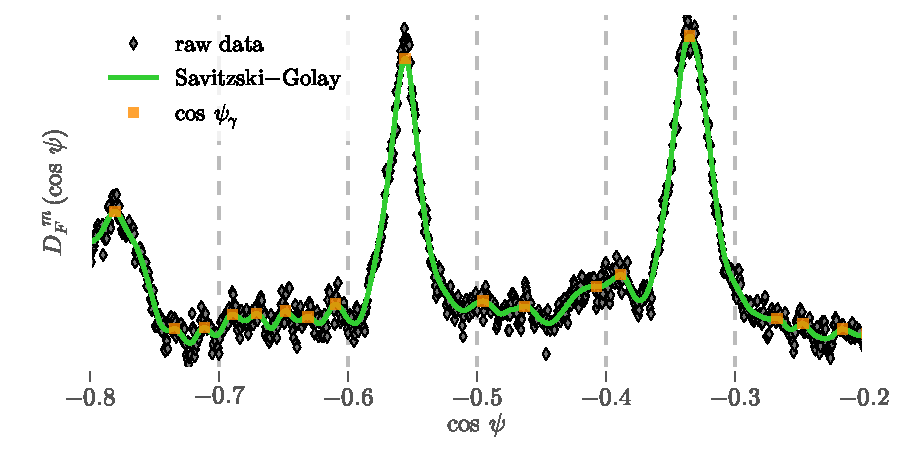
\includegraphics[]{supp_figs/peak_detection.pdf}
\caption{A portion of the angular difference correlation. Smoothing is applied, and then peaks are located by calculating local extrema.}
\label{fig:peak_detection}
\end{figure}

Then for each $\cos \psi_\gamma \in \Gamma$ we defined a Gaussian function

\be
G_\gamma (\cos \psi \,;  b,A, \eta)  =  b +  A\,\exp \left [ \frac{-\left( \cos \psi - \cos\psi_\gamma \right)^2}  {2\,\eta^2}  \right ]
\ee

The offset $b$ takes into account any residual background terms (e.g. the low-frequency background shown in Supplementary Fig. \ref{fig:compare_correlations}). The amplitude $A$ is our measure of CXS signal from the gold NPs (how far the CXS signal peaks above the background). The width $\eta$ of the CXS peak is proportional to the size of the average NP domain which scattered the correlated photons (similar to how the Bragg peak width is proportional to the size of the NP domains).

By employing the Levenberg-Marquardt non-linear least squares algorithm, we obtained the fits $(b_\gamma, A_\gamma, \eta_\gamma)$ to each detected peak. With these fits, the total fitted CXS signal can be represented by a sum of Gaussians

\be \label{fit}
G(\cos \psi) = \sum_\gamma \,\,G_\gamma ( \cos \psi \,;\, b_\gamma, A_\gamma, \eta_\gamma) - b_\gamma
\ee

Practically, we fit partial sums and optimized the parameters in parallel (Supplementary Fig. \ref{fig:gaussian_partial}).

\begin{figure}[H]
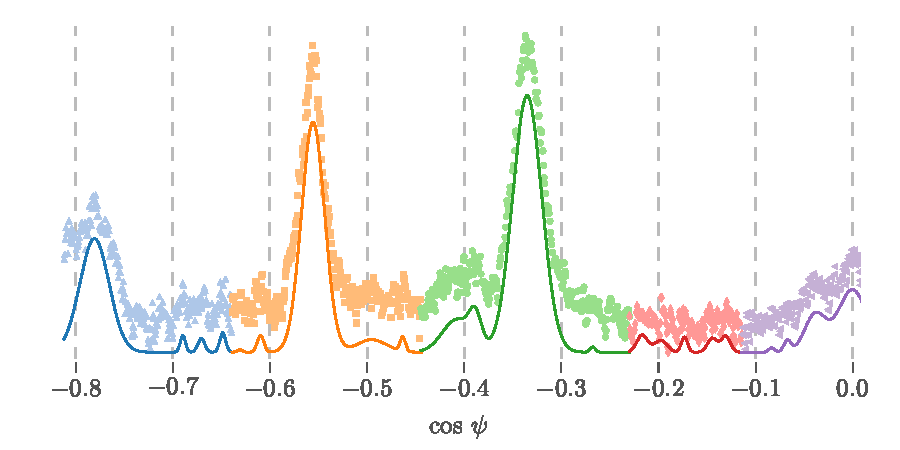
\includegraphics[scale=0.8]{supp_figs/gaussian_partial.pdf}
\caption{The symmetric difference correlation $D_F(\cos \psi)$ and partial Gaussian fits $G(\cos \psi)$ as defined in Supplementary equation (\ref{fit}). The different markers (triangle, square, circle, etc) represent different ranges over which the sum of Gaussians was fit.}
\label{fig:gaussian_partial}
\end{figure}

\section{Calculation of the signal-to-noise ratio (SNR)} \label{supp:Z}
\begin{figure}[H]
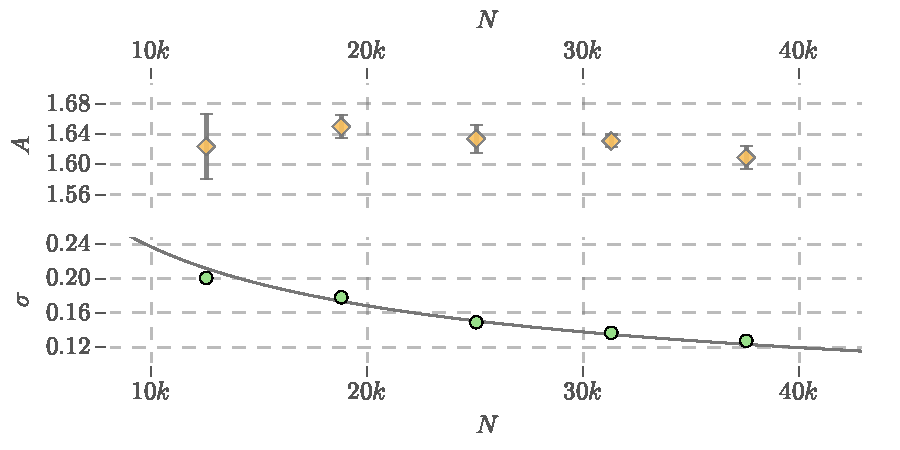
\includegraphics[]{supp_figs/new_scaling.pdf}
\caption{\emph{(Top)} The scaling and convergence of the Gaussian amplitude $A_\gamma$ for the CXS peak at $\cos \psi = 1/3$. The error bar is one standard deviation across 200 fit attempts. \emph{(Bottom)} The scaling of the CXS noise $\sigma$. The fitted curve scales as $N^{-1/2}$.}
\label{fig:scaling}
\end{figure}

We define the SNR of the Gaussian fit amplitudes $A_\gamma$ in equation (\ref{fit}) to be

\be
SNR_\gamma = \frac {A_\gamma  }{\sigma}
\ee

where $\sigma$ is estimated to be the standard deviation of the inter-difference correlation, defined as  

\be \label{ucorz}
D_{i,j,k,l}(\Delta) =\big
 \langle  \,\big(  I_i(\phi)-I_j(\phi) \big)\,\big( I_k( \phi + \Delta) - I_l( \phi+\Delta) \big) \big \rangle _{\phi}
\ee

We compute $D_{i,j,k,l}(\Delta)$  by randomly selecting pairs of exposures $i,j$ and $k,l$. If the snapshots are paired in a way that minimizes artifactual variations (see Supplementary Section \ref{pairing}), then the standard deviation of (\ref{ucorz}) is a good estimate of the theoretical noise $\sigma$ associated with a CXS measurement. This technique for noise estimation is useful in situations where CXS signal is continuous, e.g. in the case of soft matter scattering or smaller NPs with broad Bragg reflections.

Supplementary Fig. \ref{fig:scaling} shows the scaling of $A_\gamma$ and $\sigma$ for the CXS peak in $D^m_F(\cos \psi)$ at $\cos \psi_\gamma = \pm 1/3$. The fitting of $A_\gamma$ was a noisy process, especially for the lower values of $N$ when the signal level is close to the noise level. We fit multiple times until convergence of the amplitudes was reached.

\section{Estimating the size of NP scattering domains (small, twinned domains)} \label{widths_small}
From the Scherrer equation \cite{scherrer1969bestimmung} one can relate the size of a Bragg peak in reciprocal space to the size of the corresponding crystallographic domain in the NP. We define the NP size $s$ as the cube root of the domain volume. By the Schemer equation, we have 

\be \label{scherrer}
s = \frac{K \lambda}{\beta \cos \theta}
\ee 

where $K$ is a constant dependent on the shape of the domain, $\lambda$ is the photon wavelength, $\beta$ is the full-width-half-max (FWHM) of the Bragg peak in radians, and $\theta$ is half of the Bragg scattering angle at momentum transfer magnitude $q$:

\be
\theta = \arcsin \left ( \frac{q \lambda}{4 \pi} \right  )
\ee

For $\{111\}$ planes in FCC tetrahedral domains, $K \approx 0.89$ \cite{langford1978scherrer}. Typically, a Bragg peak is modeled as the convolution of a Gaussian profile (the domain size) with a Lorentzian profile (the domain strain), otherwise known as Voigt profile. By fitting Voigt profiles to Bragg peaks, one can estimate $\beta$ and hence the size of the domain which scattered the Bragg peak photons.

In the case of CXS of NPs, our assumption is that a single exposure is too noisy to measure individual Bragg peaks. However, by averaging the correlations of many exposures, we can resolve "correlated" Bragg peaks (CXS peaks) which are also related to the size of the NP domains.

A CXS peak is the average self-convolution of all correlated Bragg peaks in each exposure. Therefore, the width of the CXS peak is an approximate lower bound for the largest width of a correlated Bragg peak in the experiment. In other words, the width of the CXS peak is related to size of the smallest NP domain which scattered measurable correlated photons.

If we ignore strain contributions to the Bragg peak FWHM, $\beta$, then we can model the Bragg peak as just a Gaussian profile, and hence the CXS peak is a self-convolution of a Gaussian, which is itself a Gaussian whose width is that of the Bragg peak stretched by a factor of $\sqrt{2}$. With this, we define the FWHM of the CXS peak to be 

\be \label{gamma}
\gamma = \sqrt{2} \beta
\ee

We simulated CXS for a decahedron NP, composed of 5 identical tetrahedral domains of side length $a_{\text{sim}}\approx$ \SI{77.5}{\angstrom}. We can compute $s_{\text{sim}}$ directly as the cube root of the volume of one of the regular tetrahedra:

\be \label{smin1}
s_{\text{sim}} = \frac{ \SI{77.5}{\angstrom}} {\left( 6\sqrt{2} \right )^{1/3}} \approx \SI{38.0}{\angstrom}
\ee

We can also evaluate $s_{\text{sim}}$ using the Scherrer equation (\ref{scherrer}) combined with equation (\ref{gamma}): 

\be \label{domain_size}
s = \frac{0.89 \, \sqrt{2} \lambda}{ \gamma \cos \theta}
\ee

By fitting a Gaussian to a simulated CXS peak at $\cos \psi = {5/9}$, we find the width $\gamma_{\text{sim}} \approx \SI{0.055}{\radian}$ (see Supplementary Fig. \ref{compare_widths}), hence $s_{\text{sim}} \approx  \SI{34.7}{\angstrom}$, in agreement with Supplementary equation (\ref{smin1}).

From the difference correlation of the moderate intensities, $D^m_F(\cos \psi)$, we measure $\gamma_{\text{data}} \approx \SI{0.032}{\radian}$, corresponding to a domain size of $s^m_{\text{data}} \approx \SI{59.8}{\angstrom}$. For regular tetrahedral domains, this corresponds to a side length of

\be \label{side_length}
a^m = s^m_{\text{data}} \left(6\sqrt{2}\right)^{1/3} \approx \SI{12.2} {\nm}
\ee

For a decahedral particle composed of 5 regular tetrahedrons of side-length $a^m$, the apparent diameter can be approximated as the circumradius of the pentagon whose side-length is also $a^m$:

\be
d^m \approx a^m\,\,\frac{\sqrt{50 + 10\sqrt{5}}}{5}  \approx \SI{21.0}{\nm}
\ee   

Note, this is an approximate lower bound on the diameter of the smallest twinned NP that we measured, a conclusion we arrived at by examining the bright Bragg spots in each snapshot exposure (see Supplementary Section \ref{widths_large}).
 
\begin{figure}[H]
\includegraphics[]{supp_figs/compare_widths.pdf}
\caption{Comparing CXS peak widths at $\cos \psi = 5/9$. \emph{(Top)} The simulated CXS for a gold decahedron composed of five regular tetrahedrons of side length $a= \SI{77.5}{\angstrom}$ (diamond marker). The FWHM, $\gamma_{\text{sim}}$, corresponds to an NP domain of size $s=\SI{34.7}{\angstrom}$. The dashed line is a Gaussian fit. \emph{(Bottom)} The measured CXS (circle marker). The FWHM, $\gamma_{\text{data}}$, corresponds to an NP domain of size $s=\SI{59.8}{\angstrom}$. The solid line is a Gaussian fit.}
\label{compare_widths}
\end{figure}

\section{Estimating the size of NP scattering domains (large, non-twinned domain)} \label{widths_large}
On each image, there are Bragg rings from the gold NPs, and, on the Bragg rings, there are bright Bragg spots which appear as outliers, defined in the main text as $I^b_i(\phi)$. Because the Bragg spots are above the noise, we can measure their width and hence gather information on the corresponding domain sizes. We construct a distribution of the Bragg spot widths by performing the following steps in order:

\begin{itemize}
\item Identify the bright Bragg spots on each Bragg ring image
\item Measure the angular FWHM of the bright Bragg spots, $\beta$
\item Repeat for many images to construct a histogram
\end{itemize}

This distribution, $L(\beta)$, gives \emph{the relative number of NP domains per snapshot whose size corresponds to a Bragg spot of width $\beta$} (Supplementary Fig. \ref{fig:Lbeta}). The correlation of the bright Bragg spots, $D^b_F(\cos \psi)$,  does not show any strong signs of twinning (only having peaks at $\cos \psi = \pm 1/3$), and has peak width(s) $\gamma_{\text{outlier}} \approx \SI{0.019}{\radian}$. (One can use the distribution $L(\beta)$ to estimate $\gamma_{\text{outlier}}$ directly. For details, see Supplementary Section \ref{bragg_to_cxs}). 

A CXS peak width of $\gamma_{\text{outlier}} = \SI{0.019}{\radian}$ corresponds to an NP domain side length (assuming tetrahedral domains) of

\be
a^b = \frac{0.89\, \lambda \, \sqrt{2}\,( 6 \sqrt{2} )^{1/3} }{\gamma_{\text{outlier}} \,\cos \theta}  \approx \SI{21}{\nm}
\ee

where we made use of Supplementary equations (\ref{domain_size}) and (\ref{side_length}). Note, $a^b$ is smaller than the most commonly observed domain (that produced bright Bragg spots), whose corresponding side length we can calculate using the distribution of bright Bragg spots, 

\be
\bar{l}^{\,\,b} = \frac{0.89\, \lambda \,( 6 \sqrt{2} )^{1/3} }{ \text{argmax}\, [\,L(\beta)\,] \,\cos \theta} \approx \SI{46}{\nm}
\ee

From these results, we conclude that the CXS peak width, $\gamma_{\text{outlier}}$, corresponds to an approximate lower bound on the NP domain size in the sample.

\begin{figure}[H]
\includegraphics[]{supp_figs/Lbeta.pdf}
\caption{The distribution $L(\beta)$ of FWHM values for the bright Bragg spots measured during a single snapshot exposure. This represents the relative number of NP domains whose domain size corresponds to a FWHM of $\beta$. The bright Bragg spots are a result of the large NP domains in the sample, and the average large-domain size is the peak in this histogram, or about \SI{0.006}{\radian}. If we assume the domains are tetrahedral, this would correspond to a domain whose edge length is \SI{49}{\nm}. We note that these larger domains do not show signs of twinning.}
\label{fig:Lbeta}
\end{figure}

\subsection{Using a distribution of Bragg peak widths to estimate a corresponding CXS peak width} \label{bragg_to_cxs}
Consider that the Bragg spots are Gaussians with FWHM $\beta$. Then, as mentioned in section $\ref{widths_small}$, the correlation peak width is a convolution of two Gaussians, which is itself a Gaussian of width $\gamma = \sqrt{2}\,\beta$. Keeping in mind that we have a distribution of NP sizes (corresponding to the distribution $L(\beta)$), we can model the FWHM of the outlier correlation peak ($\gamma_{\text{outlier}}$) directly as the FWHM of the sum of Gaussians whose widths are $\sqrt{2}\,\beta$ and whose amplitudes are $L(\beta)$:

\be
G_L(\psi) = \sum_\beta L(\beta) \,\exp \left [ \frac{-\left( \psi - \arccos(1/3) \right)^2}  {2\,\sigma^2_{\gamma}}  \right ]
\ee

where $\sigma_\gamma$ is the standard deviation of the convolved Gaussian whose FWHM is $\gamma$:

\be
\sigma_{\gamma} = \frac{\gamma} {2\sqrt{2\ln{2} }} = \frac{\beta} {2\sqrt{\ln{2} }} 
\ee

The FWHM of $G_L(\psi)$ is roughly \SI{0.017}{\radian}, in good agreement with the measurement (\SI{0.019}{\radian}). 

\section{Estimating the number of NPs in each snapshot} \label{number_of_NPs}
Nanopartz Inc. provided a solution of gold NPs, each around \SI{60}{\nano \meter} across, at a concentration of \SI{100}{\mg\per\ml}. The solution reportedly contained \SI{5.21e13}{NPs per \ml}, with fewer than $0.01\%$ of NPs less than \SI{20}{\nano \meter} in diameter (according to discussions with the manufacturer). It is worth noting that our sample preparation protocol could have altered these numbers. For our experiment, we suspended the NPs in lipid cubic phase (LCP) at a concentration of \SI{40}{\mg\per\ml}. Given an exposed sample volume of \SI{1.5x2.4x 130}{\micro \meter} and a dilution factor of $0.4$, we estimate that there were roughly $9.8\cdot 10^3$ NPs exposed during each snapshot. 

\begin{thebibliography}{10}
\expandafter\ifx\csname url\endcsname\relax
  \def\url#1{\texttt{#1}}\fi
\expandafter\ifx\csname urlprefix\endcsname\relax\def\urlprefix{URL }\fi
\providecommand{\bibinfo}[2]{#2}
\providecommand{\eprint}[2][]{\url{#2}}

\bibitem{kam1977determination}
\bibinfo{author}{Kam, Z.}
\newblock \bibinfo{title}{Determination of macromolecular structure in solution
  by spatial correlation of scattering fluctuations}.
\newblock \emph{\bibinfo{journal}{Macromolecules}}
  \textbf{\bibinfo{volume}{10}}, \bibinfo{pages}{927--934}
  (\bibinfo{year}{1977}).

\bibitem{iglewicz1993volume}
\bibinfo{author}{Iglewicz, B.} \& \bibinfo{author}{Hoaglin, D.}
\newblock \bibinfo{title}{Volume 16: how to detect and handle outliers}.
\newblock \emph{\bibinfo{journal}{The ASQC Basic Reference in Quality Control:
  Statistical Technique}}  (\bibinfo{year}{1993}).

\bibitem{friedel1913symetries}
\bibinfo{author}{Friedel, G.}
\newblock \bibinfo{title}{Sur les sym{\'e}tries cristallines que peut
  r{\'e}v{\'e}ler la diffraction des rayons r{\"o}ntgen}.
\newblock \emph{\bibinfo{journal}{CR Acad Sci}} \textbf{\bibinfo{volume}{157}},
  \bibinfo{pages}{1533--1536} (\bibinfo{year}{1913}).

\bibitem{savitzky1964smoothing}
\bibinfo{author}{Savitzky, A.} \& \bibinfo{author}{Golay, M.~J.}
\newblock \bibinfo{title}{Smoothing and differentiation of data by simplified
  least squares procedures.}
\newblock \emph{\bibinfo{journal}{Analytical chemistry}}
  \textbf{\bibinfo{volume}{36}}, \bibinfo{pages}{1627--1639}
  (\bibinfo{year}{1964}).

\bibitem{scherrer1969bestimmung}
\bibinfo{author}{Scherrer, P.}
\newblock \bibinfo{title}{Bestimmung der grosse und der inneren struktur von
  kolloidteilchen mittels rontgenstrahlen (1918) in: X-ray diffraction methods
  in polymer science, ed. le alexander} (\bibinfo{year}{1969}).

\bibitem{langford1978scherrer}
\bibinfo{author}{Langford, J.~I.} \& \bibinfo{author}{Wilson, A.}
\newblock \bibinfo{title}{Scherrer after sixty years: a survey and some new
  results in the determination of crystallite size}.
\newblock \emph{\bibinfo{journal}{Journal of Applied Crystallography}}
  \textbf{\bibinfo{volume}{11}}, \bibinfo{pages}{102--113}
  (\bibinfo{year}{1978}).
\end{thebibliography}
\end{document}









